\documentclass[sn-mathphys-num]{sn-jnl}
\usepackage{graphicx} % Required for inserting images
\usepackage{amsmath}
\usepackage{float}
\usepackage{listings}
\usepackage{tikz}
\usepackage{tcolorbox}
\usetikzlibrary{shapes.geometric}
\newcommand{\warningsign}{\tikz[baseline=-.75ex] \node[shape=regular polygon, regular polygon sides=3, inner sep=0pt, draw, thick] {\textbf{!}};}
\setlength{\parskip}{\baselineskip}
\newcommand{\warning}{
	{\fontencoding{U}\fontfamily{futs}\selectfont\char 66\relax}
}

\definecolor{codegreen}{rgb}{0,0.6,0}
\definecolor{codegray}{rgb}{0.5,0.5,0.5}
\definecolor{codepurple}{rgb}{0.58,0,0.82}
% \definecolor{backcolour}{rgb}{0.95,0.95,0.92}
\definecolor{backcolour}{rgb}{1.0, 1.0, 1.0}

\lstdefinestyle{mystyle}{
		backgroundcolor=\color{backcolour},   
		commentstyle=\color{codegreen},
		keywordstyle=\color{magenta},
		numberstyle=\tiny\color{codegray},
		stringstyle=\color{codepurple},
		basicstyle=\ttfamily\footnotesize,
		breakatwhitespace=false,         
		breaklines=true,                 
		captionpos=b,                    
		keepspaces=true,                 
		numbers=left,                    
		numbersep=5pt,                  
		showspaces=false,                
		showstringspaces=false,
		showtabs=false,                  
		tabsize=2
}

\lstset{style=mystyle}

\usepackage{hyperref}

\usepackage{multicol}
\setlength{\columnseprule}{1pt}
\setlength{\columnsep}{1cm}

\usepackage{enumitem} % Required for list customization
\setlist{partopsep=0pt, topsep=0pt} % Customize spacing around and inside lists
\renewcommand{\labelenumi}{\alph{enumi}.} % Change numbering in the enumerate environment by letter rather than number

\setlength{\parindent}{0pt} % Suppress paragraph indentation

\usepackage{graphicx} % Required for including images
\graphicspath{{Figures/}{./}} % Specifies where to look for included images (trailing slash required)

\usepackage{float} % Allows more precisely positioning floats e.g. \begin{figure}[H]

%\usepackage{mhchem} % Package for chemical equation typesetting
\usepackage{siunitx} % Provides the \SI{}{} and \si{} commands for typesetting technical/scientific SI units correctly

\usepackage{amsmath, amssymb, amsthm} % Required for some math elements 

\usepackage{bookmark}
\usepackage{booktabs}

\usepackage{color}
\usepackage{tcolorbox}
\definecolor{Green}{rgb}{0.2,0.9,0.2}

\usepackage{tablefootnote}
\usepackage{amsmath, amssymb, graphics, setspace}
% \renewcommand{\labelitemi}{$\blacksquare$}

\newcommand{\mathsym}[1]{{}}
\newcommand{\unicode}[1]{{}}

\newcounter{mathematicapage}

\title[Article Title]{Rapport de Projet : Logiciel de Ray-Tracing}
% \author{Hubert Damian\\Physique BA3}
\author{\fnm{Damian} \sur{Hubert} : \sfx{Physique BA3}}
\date{Mars 2024}
% \def\imgscale{0.9}

\begin{document}
% \DeclareMathSizes{16pt}{14pt}{14pt}{14pt} 
% \setmathfont{Latin Modern Math}[Scale=10]

\setlength{\abovedisplayskip}{1pt}
\setlength{\belowdisplayskip}{1pt}

\maketitle
\tableofcontents
\section{Introduction}
La compagnie OPERA-WCG s'apprête à ouvrir de nouveaux bureaux. Le wifi n'y étant pas encore
installé, ce rapport a pour but de proposer plusieurs solutions de placement des émetteurs optimales dépendant
du budget disponible. Il commencera par la modélisation du problème avec toutes
ses hypothèses. Il décrira l'implementation logicielle
puis présentera une verification par calculs manuels. 
Finalement le rapport parlera d'optimisation et conclura sur les solutions annoncées.



\section{Modélisation}
    \subsection{Hypothèses}
    \begin{enumerate}
        \item Les rayons se propagent dans un plan horizontal $\equiv$ plan de propagation $\mathbf{\Pi}$ 
        auquel appartiendra la normale à toutes les surfaces sur lesquelles vont interagir les rayons.
        \item Le champ électrique est polarisé sur l'axe perpendiculaire à $\mathbf{\Pi}$
        donc on le considérera comme un scalaire $E$.
        \item On regarde le rayonnement de l'antenne en champ lointain (voir \ref{sub:cl}).
        \item \label{dipole} Les émetteurs sont des antennes dipoles $\lambda/2$ \textbf{sans pertes}
        et placées verticalement ($\perp \mathbf{\Pi}$) donc emission \textbf{isotrope} dans $\mathbf{\Pi}$.
        \item L'atténuation après deux réflexions est suffisante pour ne pas devoir en calculer plus.
        \item La diffraction est négligée: $\text{objets} \sim 1m >> \lambda = \frac{3.10^8ms^{-1}}{60Ghz} = 5 \times 10^{-3}m$. 
        Le tracé de rayons de l'optique géométrique s'applique.
        \item L'épaisseur des murs est negligée dans le calcul géométrique des rayons mais pas
        dans le calcul des coefficients de réflexion et de transmission.
        \item On est dans la gamme des fréquences radio où la conductivité
        peut être approximée par son expression statique $\sigma_s$
        pour ensuite définir la conductivité équivalente des matériaux par $\sigma = \sigma_s + w\epsilon^{\prime \prime}$
        traduisant la dissipation par effet Joule et diélectrique.
        \item La puissance est calculée en zone locale (puissance moyenne).
    \end{enumerate}

    \subsection{Formules}

    On calculera la puissance dans une zone locale par
    \begin{align}
        <P_{R X}>=\frac{1}{8 R_a} \sum_{n=1}^N\left|\vec{h}_e^{R X}\left(\theta_n, \phi_n\right) \cdot \underline{\vec{E}}_n(\vec{r})\right|^2\\
        \underline{E}_n=\underbrace{\Gamma_1 \Gamma_2 \ldots}_{\text {Réflexions }} \underbrace{T_1 T_2 \ldots}_{\text {Transmissions }} E_0\left(\theta_{T X n}, \phi_{T X n}\right) \frac{e^{-j \beta d_n}}{d_n}
    \end{align}
    La propriété d'isotropie de l'antenne dans $\mathbf{\Pi}$ permet de définir la constante $P_{RX0} = \frac{60 G_{RX}P_{RX} \lambda^2}{8 R_{ar} \pi^2}$ avec
    $G_{RX}P_{RX} = \frac{Z_0 P_{TX}}{\pi R_{ar}}$ et on obtient
    \begin{equation}
    \label{f:p_moy}
        <P_{RX}> = P_{RX0} \sum_{n=1}^N |\Gamma_1|^2 \dots |T_1|^2 \dots \frac{1}{d_n^2}
    \end{equation}

    Le reste des formules sera vu dans l'exercice $\ref{subsub:2rebond}$

    \subsection{Champ lointain}
    \label{sub:cl}

    Il faut prendre des précautions avant d'appliquer l'hypothèse des
    champs lointains. 

    Il faut se trouver à une distance $d > d_{\mathrm{ff}}$
    \begin{equation}
        d_{\mathrm{ff}}=\operatorname{Max}\left\{1,6 \lambda ; 5 D ; \frac{2 D^2}{\lambda}\right\}
    \end{equation}
    Avec une antenne dipole : $D = \frac{\lambda}{2}$ et donc \fbox{$d_{\mathrm{ff}} = 5\frac{\lambda}{2}=12.5mm$}

    Dans le code cela sera pris en compte dans la puissance maximale
    admise pour le trajet de chaque rayon. 
    Dans la fonction \texttt{calculate\_power} de \textbf{unit\_solver},
    avant de multiplier par les coefficients $T, \Gamma$ on s'assure que 
    $\frac{P_{RX0}}{d_n^2} < \frac{P_{RX0}}{d_{\mathrm{ff}}^2}$.

 
\section{Fonctionnement du code}
\subsection{Architecture générale}

\begin{figure}[H]
    \centering
    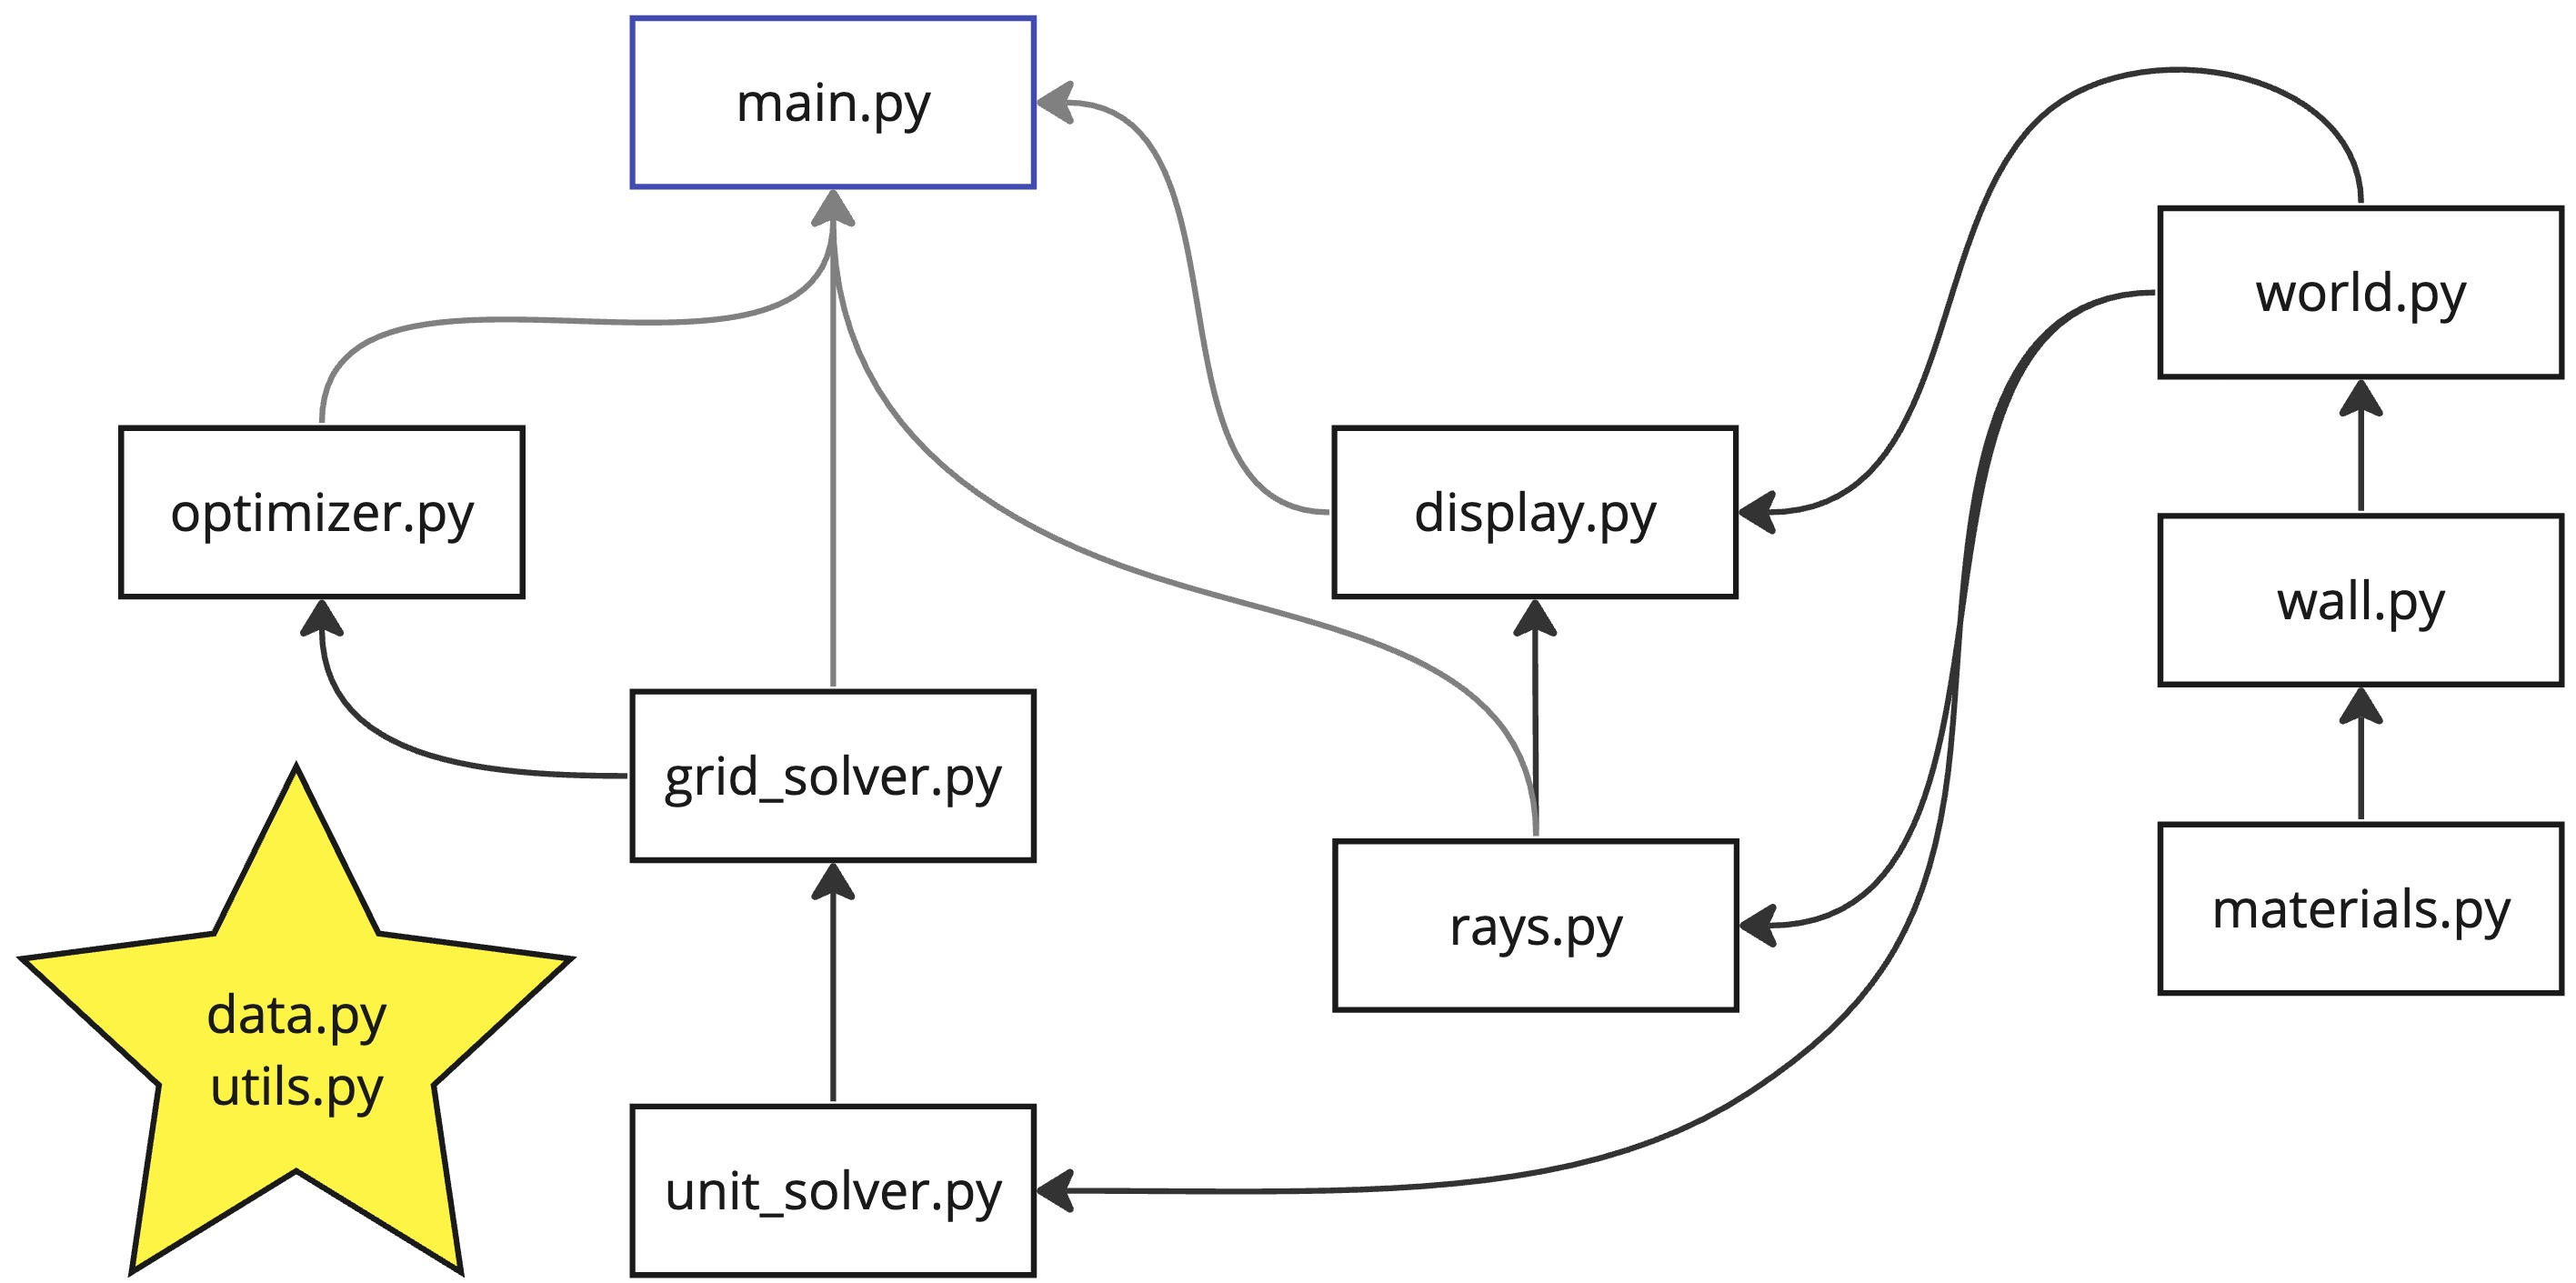
\includegraphics[width=0.7\textwidth]{images/programme.jpeg}
\end{figure}

\subsection{World}

L'objet \textbf{world} contient tous les \textbf{wall} d'abord en mémoire dynamique provisoire
puis transférée dans le gpu.

Chaque objet \textbf{wall} contient ses coordonnées, ses vecteurs unitaires $\vec{u}$ (tangent)
et $\vec{n}$ (normal) et une instance du \textbf{material} le décrivant.
Cet objet \textbf{material} contient les propriétés $\epsilon_r, \sigma$ et pré-calcule $Z, \gamma$.

La classe \textbf{Wall} contient des méthodes \texttt{@static} pour calculer les coefficients
de réflexion $\Gamma$ et de transmission $T$ en module carré.

\subsubsection{Optimisation: AoS vs SoA}
Une fois le transfert dans le gpu achevé, 
\textbf{world} va contenir ses \textbf{wall} sous forme 
d'\texttt{arrays} et non sous forme d'objets.
Par exemple les normales de tous les murs seront dans une grande array.
Un mur sera juste un indice dans ces grandes \texttt{arrays}.

Si on arrange mal notre mémoire on peut augmenter le taux de \textit{cache miss}.

Par exemple, si on demande la normale au mur 3, il est fort probable
que l'on demande aussi son vecteur tangent, ses coordonnées, etc. 
Il serait pratique d'avoir ses informations stockées proches 
les unes des autres.
C'est pourquoi nous utilisons un stockage \texttt{AoS : array of structures}
plutôt que \texttt{SoA : structure of arrays}
% \begin{lstlisting}[language=python,title=https://docs.taichi-lang.org/docs/layout]
\begin{lstlisting}[language=python]
# address: low ...................... high
# AoS:     RGBRGBRGBRGBRGBRGB.............
# SoA:     RRRRR...RGGGGGGG...GBBBBBBB...B    
\end{lstlisting}

On accomplit cela dans le code au moment d'allouer la mémoire dans 
des \texttt{dense fields} de taichi
\begin{lstlisting}{language=python}
    ti.root.dense(ti.i, self.m).place(self.r0, self.r1, self.u, self.n, self.l, self.gamma, self.Z, self.eps_r)
    # instead of 
    # ti.root.dense(ti.i, self.m).place(self.r0)
    # ti.root.dense(ti.i, self.m).place(self.r1)
    # and ...
    # which would give us a SoA
\end{lstlisting}

Bien que beaucoup de murs partagent leur matériaux en communs,
ceux-ci ont été dupliqués. Cela a rendu le code plus simple (car accès à toutes les propriétés du mur par un indice) 
et à peut être aussi rendu l'accès mémoire plus localisé mais ça n'a
pas été vérifié.


\subsubsection{Optimisation sur le calcul des angles}

Passer par les fonctions trigonométriques $\arccos$ puis $\cos$ et $\sin$
est lent pour l'ordinateur.

\textbf{Wall} ne calcule donc pas les angles mais plutôt les fonctions trigonométriques
directement comme montré dans l'exemple \ref{subsub:2rebond}.

\subsection{Unit Solver}

Le fichier \textbf{unit\_solver} contient les méthodes pour calculer la puissance moyenne qu'on
obtiendra en un point $rx$ depuis un point $tx$ en calculant chaque réflexion et transmission de tous les rayons possibles.

\subsubsection{Transmission}

Une fonction \texttt{find\_intersection(r0, u, p2, q2)} pour trouver l'intersection entre
un mur et un rayon en renvoyant un paramètre $t$ qui donne le point par $\vec{r} = t \vec{u}$.
\warningsign ce paramètre ne garantit pas encore que l'on a une intersection physique.
Pour cela, il faut passer à la fonction suivante: \texttt{intersect(u, n, p1, q1, p2, q2)}
(avec p1, q1 les points extrêmes du mur et q2, p2 le rayon). 
Dans cette fonction on vérifie d'abord que p2 et q2 soient chacun d'un côté different du mur grâce
 à leur produit scalaire avec $\vec{n}$, 
puis on regarde le point d'intersection ip et on determine par $sign(<ip-p1,u>) ?= sign(<ip-q1,u>)$ 
si il fait partie du mur ou non.

On peut maintenant définir \texttt{wall\_transmission(world, p2, q2, index1=-1, index2=-1)}
qui va prendre un rayon et itérer parmi tous les murs pour déterminer avec la fonction
\texttt{intersect} si il faut calculer un coefficient de transmission (par la fonction dans \textbf{Wall}). Dans
ce cas, il sera multiplié au coefficient global de transmission renvoyé par la fonction.
Si l'on sait que le rayon part d'un mur ou rebondit sur un mur, \texttt{index1,2} permet 
de les enlever de la boucle.

\subsubsection{Reflexion}
Avant de traiter les réflexions, on prévoit la fonction \texttt{bounce\_cond(r0, n, tx, rx)}
pour vérifier l'existence physique de cette dernière par rapport au mur avec
$sign(<n,p2 - r0>) ?= sign(<n,q2 - r0>)$ ($r0$ un point du mur et $p2,q2$ le rayon)


\subsubsection{Mise en commun}
En mettant ces fonctions en commun, on arrive à la fonction 
principale \texttt{calculate\_power(world, tx, rx)} dont
le but va être de remplir la formule \eqref{f:p_moy}.

\begin{enumerate}
    \item[0] Elle calcule d'abord la
composante directe avec \texttt{wall\_transmission} et la distance entre $tx$ et $rx$
    \item[1] Puis on passe au premier itérateur des murs: au sein de celle-ci,
on utilise le tracé géométrique pour obtenir le trajet, on vérifie si la réflexion
est physique avec \texttt{bounce\_cond}, on trouve le point d'intersection avec
\texttt{find\_intersection},
on vérifie par une méthode analogue à celle dans \texttt{intersect} si ce point fait partie du mur.
Et enfin on calcule les coefficient de transmission de chaque rayon avec \texttt{wall\_transmission}
et les coefficient de réflexion pour chaque rayon avec la méthode statique \texttt{Wall.get\_rn2} (module carré).
    \item[2] On place dans ce premier itérateur le deuxième pour traiter des réflexions doubles.
On vérifie d'abord qu'on ne fait pas une réflexion double sur le même mur.
Ensuite, le tracé géométrique demandant d'abord le calcul du dernier (deuxième) point d'intersection,
on procède aux mêmes vérifications et calculs en marche arrière jusqu'à retomber sur $tx$
puis de calculer les coefficients pour chaque rayon.
\end{enumerate}


\begin{tcolorbox}[colback=red!10!white,colframe=red!50!black,title=Remarque,sharp corners]
    L'exécution d'un code dans le gpu rend la définition d'un algorithme récursif inutile.
    Étant donné que la récursion n'est pas disponible, 
    pour une fonction de récursion qui se rappelle n fois, le compilateur
    devrait générer et compiler une fonction non récursive pour chaque changement de n.
    Le nombre de réflexions étant seulement de 2, il n'est pas grave d'expliciter le tout en 2 for-loops.
\end{tcolorbox}

\subsection{Grid}

La classe Grid parallelise \texttt{calculate\_power} de \textbf{unit\_solver} sur une grille 3D de $rx$ pour $n$ émetteurs.
La puissance moyenne est donc calculée pour tous ses points. On sélectionne
ensuite la puissance maximale parmi les $n$ émetteurs. Ceci fait, on peut convertir
le tout en $dbm$ et en débit binaire.

\subsubsection{Conversion en débit binaire}
\label{subsub:conversion_bin}

On a une relation linéaire de la puissance en $dbm$ vers le débit binaire en $\log$.

On construit donc une fonction pour passer de l'un à l'autre qui ne devrait
 être utilisée que dans la gamme (-90dbm à -40dbm).

% \begin{table}[H]
\begin{table}[htbp]
\centering
\begin{tabular}{|ccc|}
    \hline Sensibilité & Débit binaire & log(Débit binaire) \\
    \hline$-90 \mathrm{dBm}$ & $50 \mathrm{Mb} / \mathrm{s}$ & 6 + log(50) \\
    \hline$-40 \mathrm{dBm}$ & $40 \mathrm{~Gb} / \mathrm{s}$ & 9 + log(40) \\
    \hline
\end{tabular}
\end{table}

\begin{align*}
    &f \colon x \in [-90, -40] \longrightarrow 6 + \log(50) + \frac{3 + \log(40) - \log(50)}{50} (x + 90)\\
    &\text{débit binaire} = 10^{f(x)}
\end{align*}

\subsubsection{Optimisation par la librairie Taichi}
La librairie python \texttt{taichi} permet d'une part de compiler des fonctions
python en langages plus rapide et d'autre part de paralléliser
les for-loop au scope d’exécution le plus haut dans les fonctions ayant le décorateur
\texttt{@ti.kernel}. La compilation et l'exécution en parallèle dans le cpu permettent
déjà d'atteindre l'ordre de $10^{-2}s$ puis avec le passage au gpu : $10^{-3}s$ pour une grille
de cellules $10cm\times10cm$ sur le plan de OPERA-WCG. Ces calculs sont effectués sur une
puce m1 pro qui se situe selon les benchmark entre une Nvidia GeForce RTX 3050 Ti (Laptop) et 4050 (Laptop)\footnote{\href{https://www.notebookcheck.net/Apple-M1-Pro-14-Core-GPU-Benchmarks-and-Specs.576651.0.html}{notebookcheck.net benchmark}}

Dans ce temps de calcul, on compte aussi le temps pour pouvoir utiliser les données en dehors du contexte de taichi
sans quoi il semblerait que l'on puisse descendre encore un peu sur le
temps d'exécution pour l'option gpu (l'option cpu ne souffrant pas de ces transferts de données).
L'idéal aurait alors été de centrer la conception du programme autour de l'algorithme d'optimisation
pour éviter ces transfers gpu-cpu. Cela aurait néanmoins empêché d'utiliser une 
librairie externe d'algorithmes d'optimisation et aurait rendu le développement bien plus long.
La temps d'exécution étant bien assez court, cela n'a pas été requis.

\subsubsection{Optimisation: pourquoi paralléliser sur la grille de rx ?}
Une autre option aurait été de paralléliser le calcul sur la double for-loop de \texttt{calculate\_power} directement.
Seulement, on cherche à paralléliser le plus d'éléments possibles et si on compare ces deux options:
\begin{itemize}
    \item 17 murs, double for-loop : $\rightarrow 17^2 = 289$
    \item grille de $0.5m$ minimum, calcul en tout point de la grille : $\rightarrow \frac{8}{0.5} \times \frac{15}{0.5} = 480$
    (sans compter le facteur $n$ pour les émetteurs)
\end{itemize}

Il est donc preferable de paralléliser sur la grille.





\subsection{Data \& Utils}
data.py \& utils.py sont partagés par tous les fichiers, 
ils contiennent d'une part toutes les données pour
caractériser le problème et d'autre part des imports et méthodes souvent utilisés

Les données introduites dans le logiciel pour OPERA-WCG et pour le problème illustratif
du syllabus d'exercice sont dans l'annexe \ref{sub:data}

\subsection{Affichage}
\textbf{display} s'occupe de plot les données de la grille dans un repère orthonormé. Il peut faire appel à \textbf{Rays}
qui contient tous les rayons à (0,1,2) rebonds pour un couple $(tx,rx)$ donné.

L'objet \textbf{display} fera aussi appel à \textbf{world} pour qu'il utilise \textbf{display}
pour dessiner les murs avec le code couleur de la table \ref{tab:code_couleur}.

\begin{table}[htbp]
    % \centering
    \caption{Code couleur}
    \label{tab:code_couleur}
    
\begin{tabular}{|c|c|c|c|} 
    \toprule
    Matériaux & $\epsilon_r$ & $\sigma[S/m]$ & couleur \\
    \midrule
    % Brique & 3,95 & 0,073 & \textcolor{}{} \\
    % \midrule
    Béton & 6,4954 & 1,43 & \textcolor{red}{$\blacksquare$}\\
    \midrule
    Cloison & 2,7 & 0,05346 & \textcolor{green}{$\blacksquare$}\\
    \midrule
    Vitre & 6,3919 & 0,00107 & \textcolor{cyan}{$\blacksquare$}\\
    \midrule
    Paroi métallique  & 1 & $10^7$ & \textcolor{gray}{$\blacksquare$} \\
    \bottomrule
\end{tabular}
\end{table}

Il y aura 2 affichages :
\begin{itemize}
    \item Affichage de la puissance moyenne en $dbm$ bornée de $-40dbm$ à $-90dbm$
    (on transforme tout ce qui est en dessous de $-90dbm$ en $-\infty \equiv 0W$)
    \item Affichage du débit binaire en $GB/s$ par \ref{subsub:conversion_bin}.
\end{itemize}




\section{Vérification}

\subsection{Exercice du syllabus}
\begin{figure}[H]
    \centering
    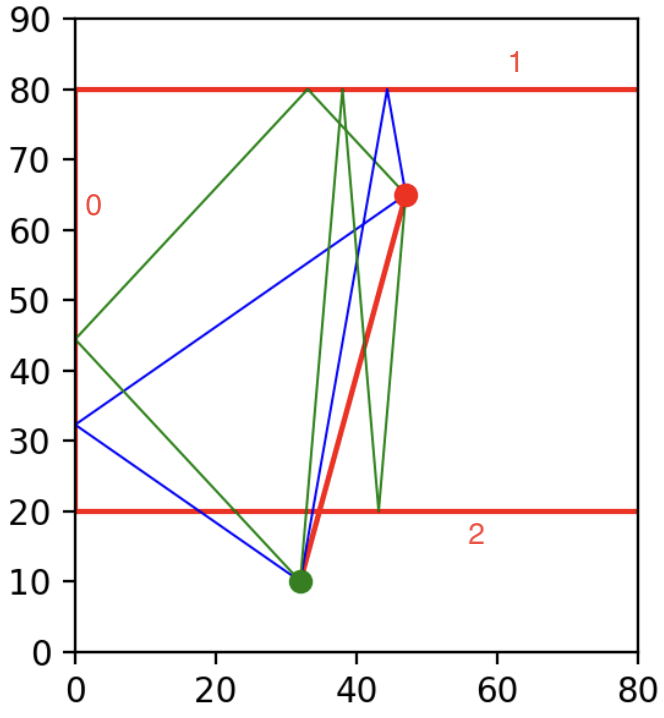
\includegraphics[width=0.35\textwidth]{images/verif/rayons.png}
    \caption{Sortie graphique du programme quand on entre les données de l'exercice. Les axes sont en [m]. \textbf{Les murs sont nommés de 0 à 2}}
    \label{f:ray_ex}
\end{figure}

\begin{figure}[H]
\begin{lstlisting}[language=python]
direct : Prx 3.336E-10 <-
first bounce : wall 0 : Prx 1.039E-11 <-
second bounce : wall 0,1 : Prx 4.136E-12 <-
first bounce : wall 1 : Prx 9.554E-12
second bounce : wall 1,2 : Prx 1.287E-13
total rays: 5
\end{lstlisting}
\caption{\texttt{stdout} du programme quand on entre les données de l'exercice}
\end{figure}

On utilise ici la classe \textbf{Rays} pour le calcul, car celle ci
possède une fonction \texttt{calculate\_power} modifiée pour stocker les
points de rayons et afficher les puissances partielles (pour chaque composante à (0,1 ou 2) réflexions)

Les paramètres pour ce problème sont en commentaire dans l'annexe \ref{sub:data}.
\subsubsection{Calcul pour un exemple à deux rebonds}
\label{subsub:2rebond}

Les formules importantes ont été écrites dans \textit{mathematica} pour faciliter
le calcul avec les nombres complexes. 

\begin{figure}[H]
    \centering
    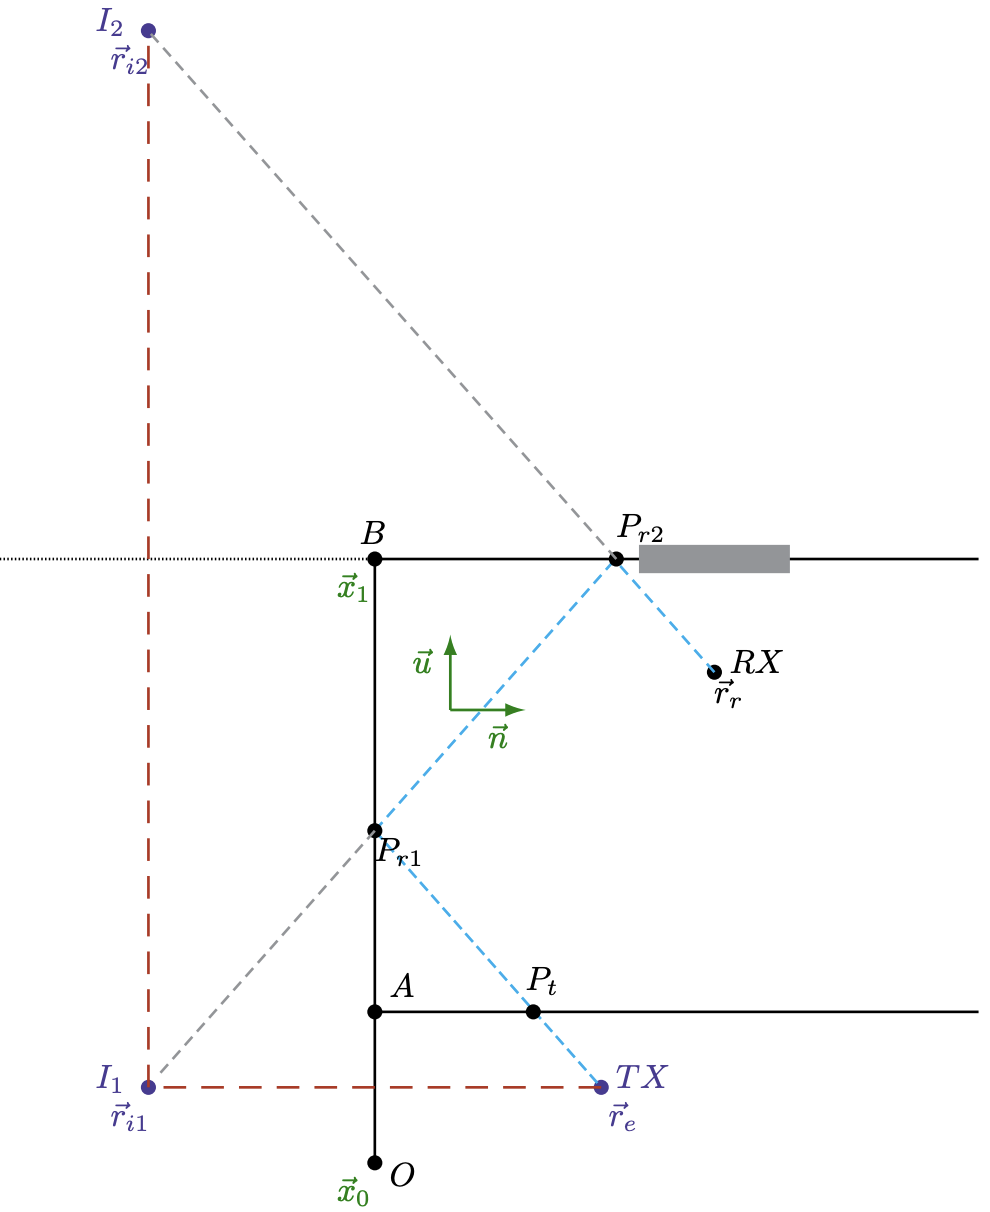
\includegraphics[width=0.4\textwidth]{images/verif/2_rebonds.png}
    \caption{Tracé géométrique du problème, $tx = (32, 10)$ et $rx = (47, 65)$}
    \label{f:exemple}
\end{figure}

On commence par trouver géométriquement les points $\vec{r}_{i1}, \vec{r}_{i2}$

\begin{align*}
    &\vec{r}_{i1} = (-32, 10) &\vec{r}_{i2} = (-32, 150)
\end{align*}

On voit qu'on aura une transmission en $Pt$ et 2 réflexions en $Pr1, Pr2$

On doit trouver ces points d'intersection avec les murs.
Pour cela il suffit de faire une interpolation linéaire de 2 points du rayons
et de regarder le point $x$ ou $y$ pour lequel on intersecte le mur.
La connaissance de $Pt$ requiert la connaissance de $Pr1$ qui lui même requiert $Pr2$.

Commençons donc par $Pr2$:
On fait une interpolation linéaire de $\vec{r}_{i2}$ à $\vec{r}_{r}$ $\equiv f(x)$

\begin{align*}
    &f(x) = y_{i2} + \frac{y_r - y_{i2}}{x_r - x_{i2}}(x - x_{i2})
    = 150 - \frac{85}{79}(x + 32)\\
    &\textrm{on cherche $x$ pour avoir $y=f(x)=y_{mur1}=80$}\\
    &f(x) = 80 \iff x = 33.05 = x_{Pr2}
\end{align*}

Finalement : $Pr2 = (33.05, 80)$

On peut effectuer des calculs presque identiques et obtenir $Pr1 = (0, 44.435)$ et $Pt = (22.707, 20)$

Il ne reste qu'à calculer les angles d'incidence $\cos(\theta_i), \sin(\theta_i)$ 
et de transmission $\cos(\theta_t), \sin(\theta_t)$
avant de pouvoir calculer les coefficients de transmission et de réflexion.

Commençons par les angles de la transmission sur le mur 2 (voir figure \ref{f:ray_ex})

\begin{equation}
\label{f:cos_i}
    \begin{aligned}
    & \cos \theta_i=\left|<\frac{\vec{d}}{\|d\|}, \vec{u}>\right|=\frac{d_y}{\|d\|}=0.732532
    \end{aligned}
\end{equation}
Dans cette formule \eqref{f:cos_i}, on a pris $\vec{u}$ pour avoir
le vecteur normal à la surface du mur et on a défini un vecteur
d'incidence $\vec{d} = Pr1 - \vec{r}_e$

$\sin(\theta_i)$ est obtenu simplement par $\sqrt{1 - \cos(\theta_i)^2} = 0.680733$

Ensuite l'angle de la transmission dans le mur est donné par $\sin(\theta_t) = \frac{\sin(\theta_i)}{\sqrt{\epsilon_r}} = 0.31071$
et $\cos(\theta_t) = \sqrt{1 - \sin(\theta_t)^2} = 0.950505$

Le coefficient de réflexion de surface pour une polarisation perpendiculaire

\begin{equation}
    \Gamma_{\perp}\left(\theta_i\right)=\frac{Z_m \cos \theta_i-Z_0 \cos \theta_t}{Z_m \cos \theta_i+Z_0 \cos \theta_t} = -0.48052 + 0.014901j 
\end{equation}

On définit $s = \frac{l}{cos(\theta_t)} = 0.157811$ la distance parcourue dans le mur.

\begin{equation}
    T_m\left(\theta_i\right)=\frac{\left(1-\Gamma_{\perp}^2\left(\theta_i\right)\right) e^{-\gamma_m s}}{1-\Gamma_{\perp}^2\left(\theta_i\right) e^{-2 \gamma_m s} e^{j \beta 2 s \sin \theta_t \sin \theta_i}}=
    0.62948 + 0.0890456j
\end{equation}

On calcule de manière similaire les paramètres pour les 2 réflexions en utilisant
\begin{equation}
    \Gamma_{m}\left(\theta_i\right)=\Gamma_{\perp}\left(\theta_i\right)-\left(1-\Gamma_{\perp}^2\left(\theta_i\right)\right) \frac{\Gamma_{\perp}\left(\theta_i\right) e^{-2 \gamma_m s} e^{j \beta 2 s \sin \theta_t \sin \theta_i}}{1-\Gamma_{\perp}^2\left(\theta_i\right) e^{-2 \gamma_m s} e^{j \beta 2 s \sin \theta_t \sin \theta_i}}
\end{equation}
\begin{align}
    &\Gamma_{m,1} = -0.471151 + 0.251816j 
    &\Gamma_{m,2} = -0.419027 + 0.246183j
\end{align}

On voit géométriquement (figure \ref{f:exemple}) que la distance est $|\vec{r}_r - \vec{r}_{i2}|$ et en utilisant la formule \eqref{f:p_moy}:

\begin{align}
    <P_{RX}> = P_{RX0} \times |T_{m}|^2 \times |\Gamma_{m,1}|^2 \times |\Gamma_{m,2}|^2 \frac{1}{d^2} = 4.127 \times 10^{-12}
\end{align}

\subsubsection{Vérification avec le code}

Dans l'exercice du syllabus, vu qu'on calcule les champs, on obtient des phénomènes 
d'interference non présents dans la puissance moyenne. Il faut donc
faire attention à bien prendre les résultats qui utilisent la puissance moyenne.

\begin{table}[htbp]
    \centering
    \caption{Vérification des puissances moyennes [W]}
    \label{tab:my_table}
    \begin{tabular}{c|c|c}
        \toprule
        Murs & Puissance Syllabus ou Calculée & Puissance Code \\
        \midrule
        direct $\times$ & $3.33 \times 10^{-10}$ & $3.336 \times 10^{-10}$ \\
        une réflexion avec 0 & $1.039 \times 10^{-10}$ 
        \tablefootnote{Dans le syllabus on a le résultat en $dBm$ de la puissance moyenne
            comptant la transmission directe et le premier rebond sur le mur 0.
            En passant en $W$ et en soustrayant la composante directe, on obtient bien
            le résultat affiché
        } & $1.039 \times 10^{-10}$ \\
        deux réflexions avec 0 puis 1 & $4.127 \times 10^{-12}$ & $ 4.136 \times 10^{-12} $\\

        % Fill in your data here
        \bottomrule
    \end{tabular}
\end{table}

\subsection{Vérification du tracé des rayons}

On se place dans le cas un peu plus complexe des bureaux de OPERA-WCG.

\begin{figure}[H]
    \centering
    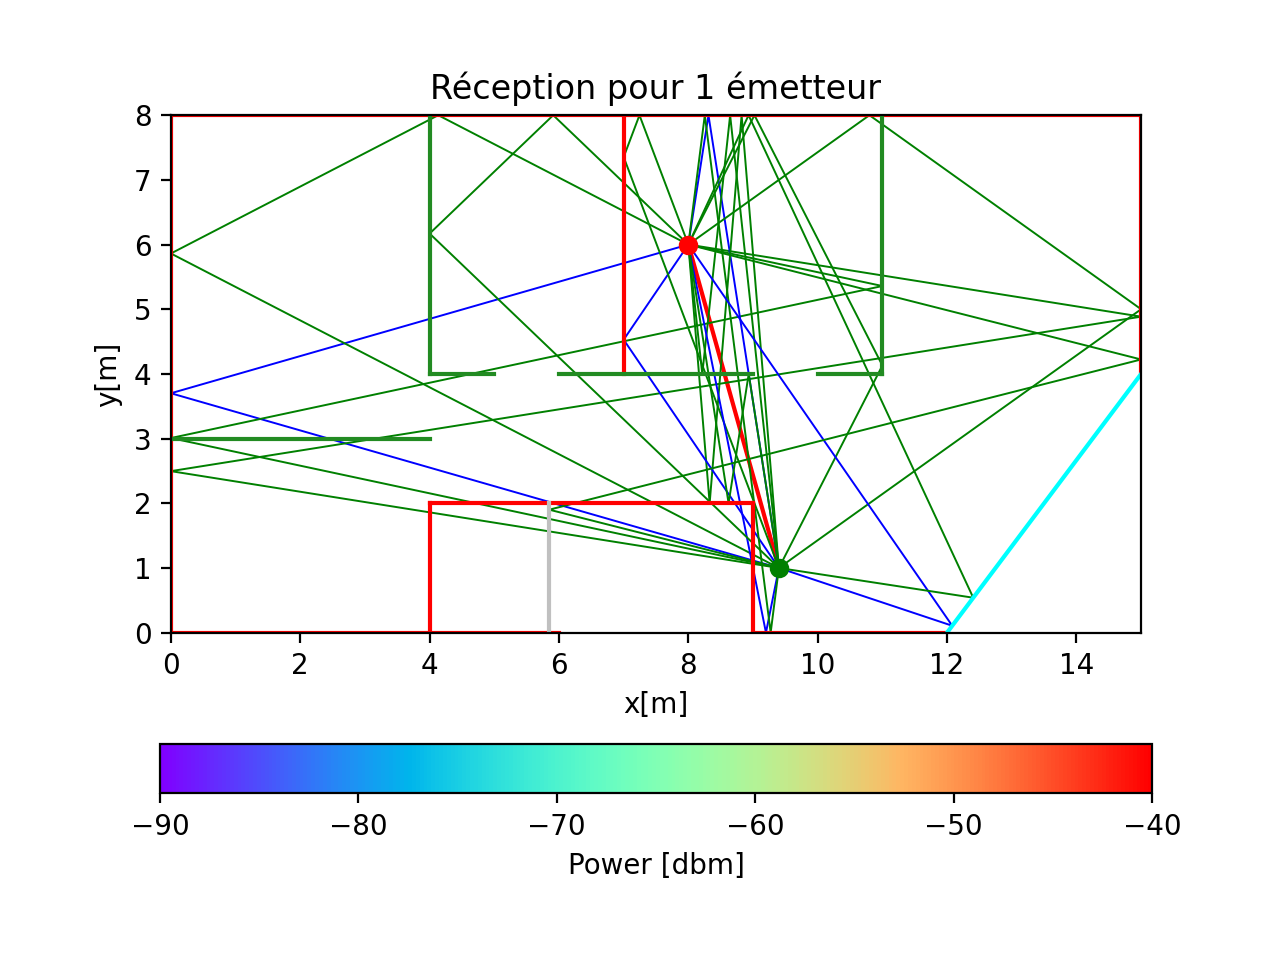
\includegraphics[width=0.7\textwidth]{images/verif/rayons_complex.png}
    \caption{tx = (9.4, 1.0), rx = (8.0, 6.0)}
\end{figure}

\begin{figure}[H]
    \centering
    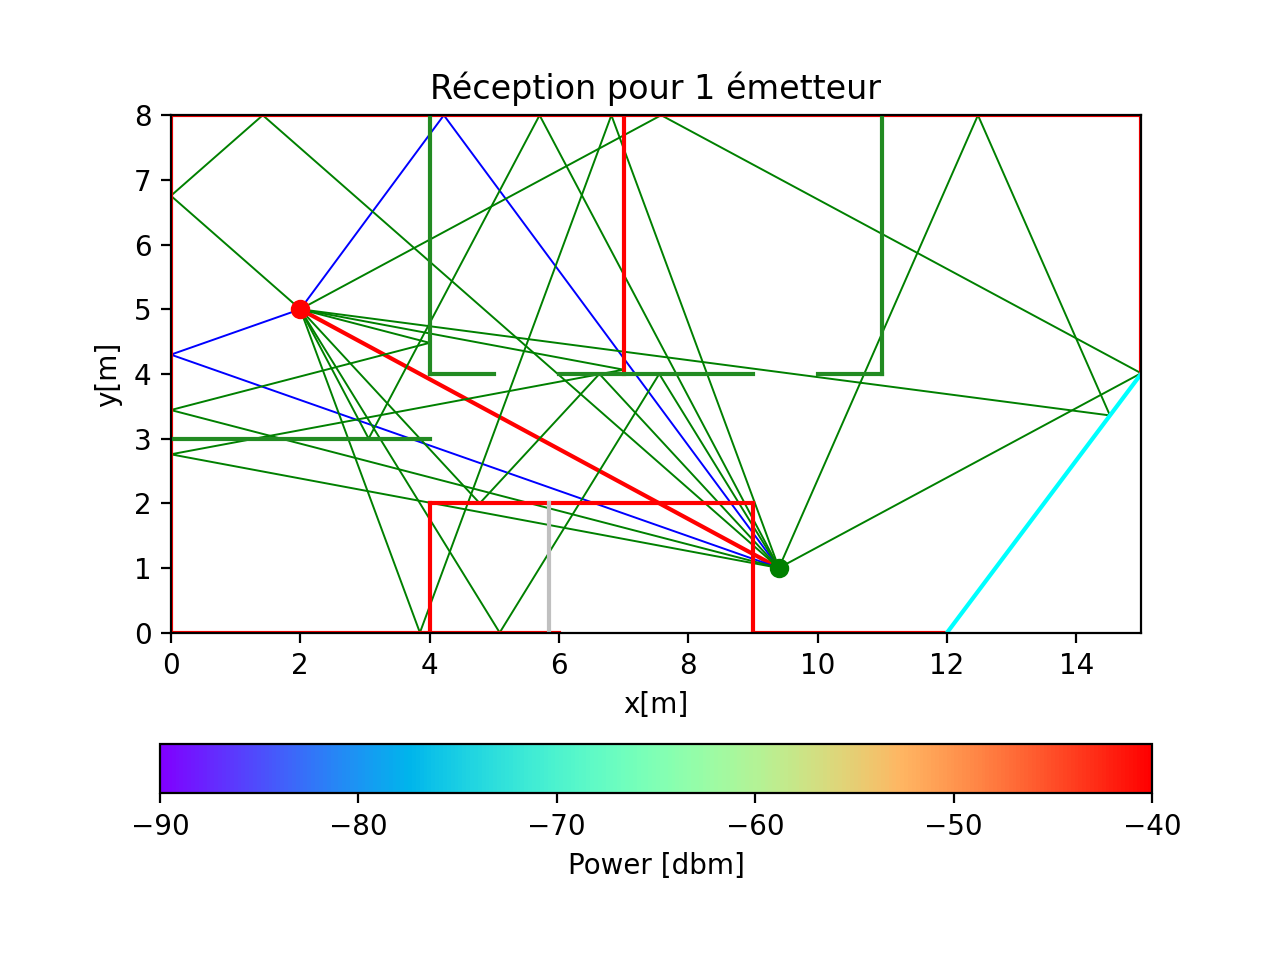
\includegraphics[width=0.7\textwidth]{images/verif/rayons_complex_2.png}
    \caption{tx = (9.4, 1.0), rx = (2.0, 5.0)}
\end{figure}

Tous les rayons semblent être explicables par l'optique géométrique.
    

\section{Résultat de calcul}

Pour les bureaux d'OPERA-WCG on obtient la figure \ref{fig:base}
\begin{figure}[H]
    \centering
    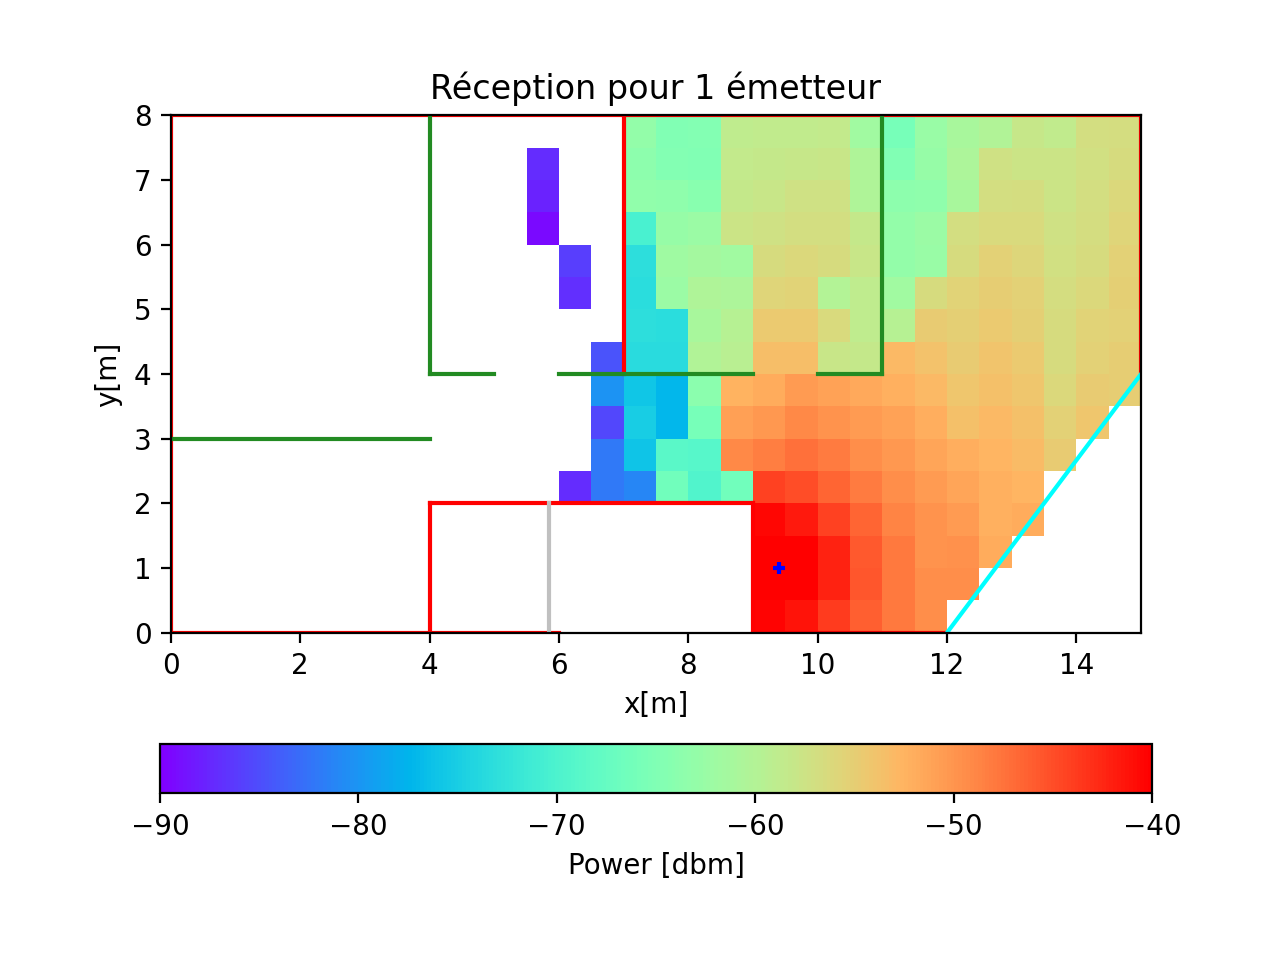
\includegraphics[width=0.49\textwidth]{images/1_dbm_non_opti.png}
    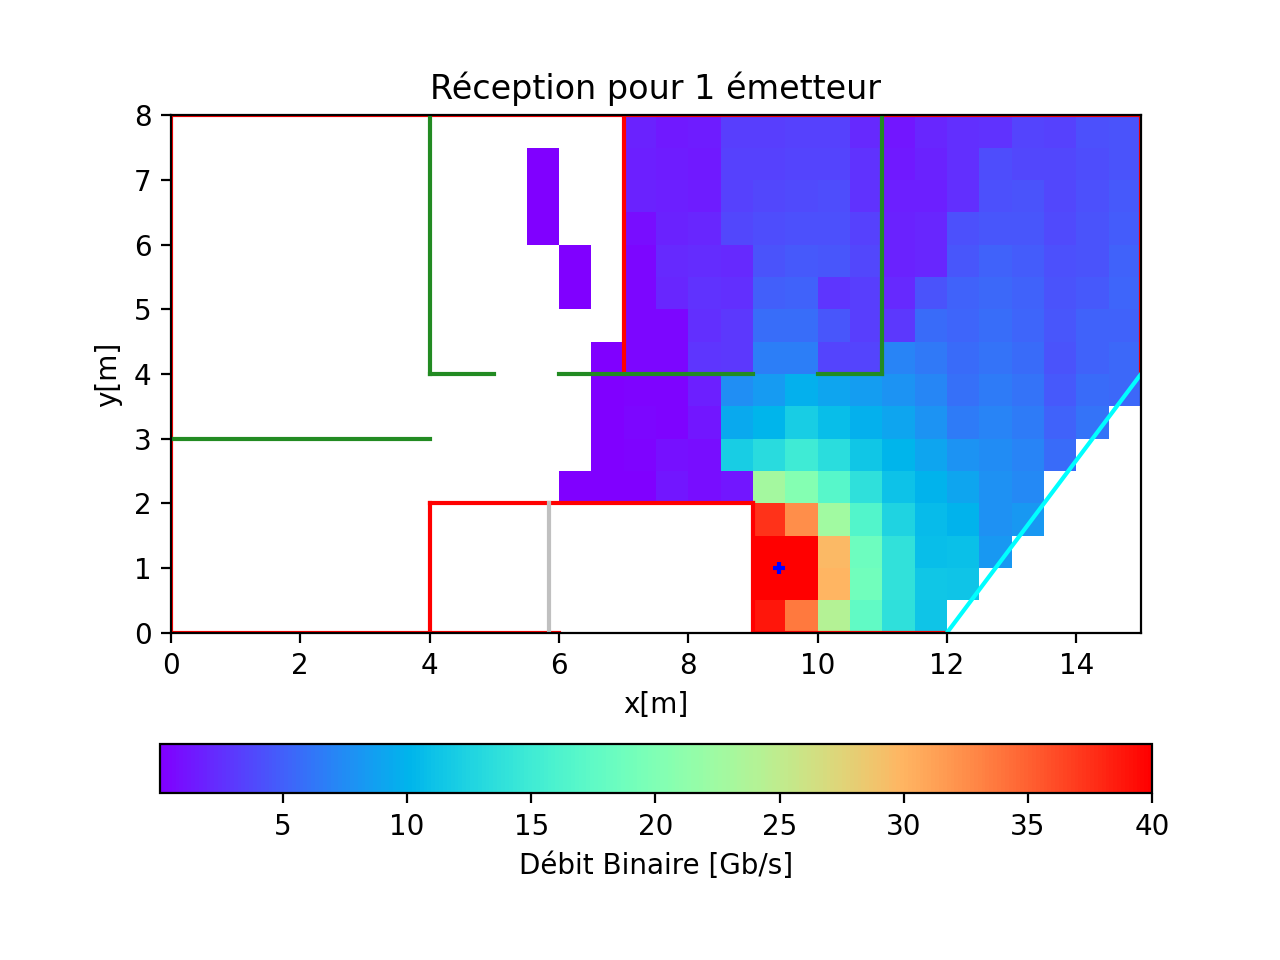
\includegraphics[width=0.49\textwidth]{images/1_bin_non_opti.png}
    \caption{Émetteur dans la position suggérée : tx = (9.4, 1.0); grille de pas 0.5m}
    \label{fig:base}
\end{figure}

La profondeur de peau de notre béton à cette fréquence : $\delta = \frac{1}{105.63} < 1cm$.
Les murs ayant une épaisseur de 30cm, il n'y aura jamais aucune onde qui passera au travers
pour atteindre l'ascenseur.
On supposera donc que l'ascenseur n'est pas présent pour réduire le temps de calcul. 
La figure \ref{fig:elevator} montre effectivement que cet ascenseur n'a pas d'impact.

\begin{figure}[H]
    \centering
    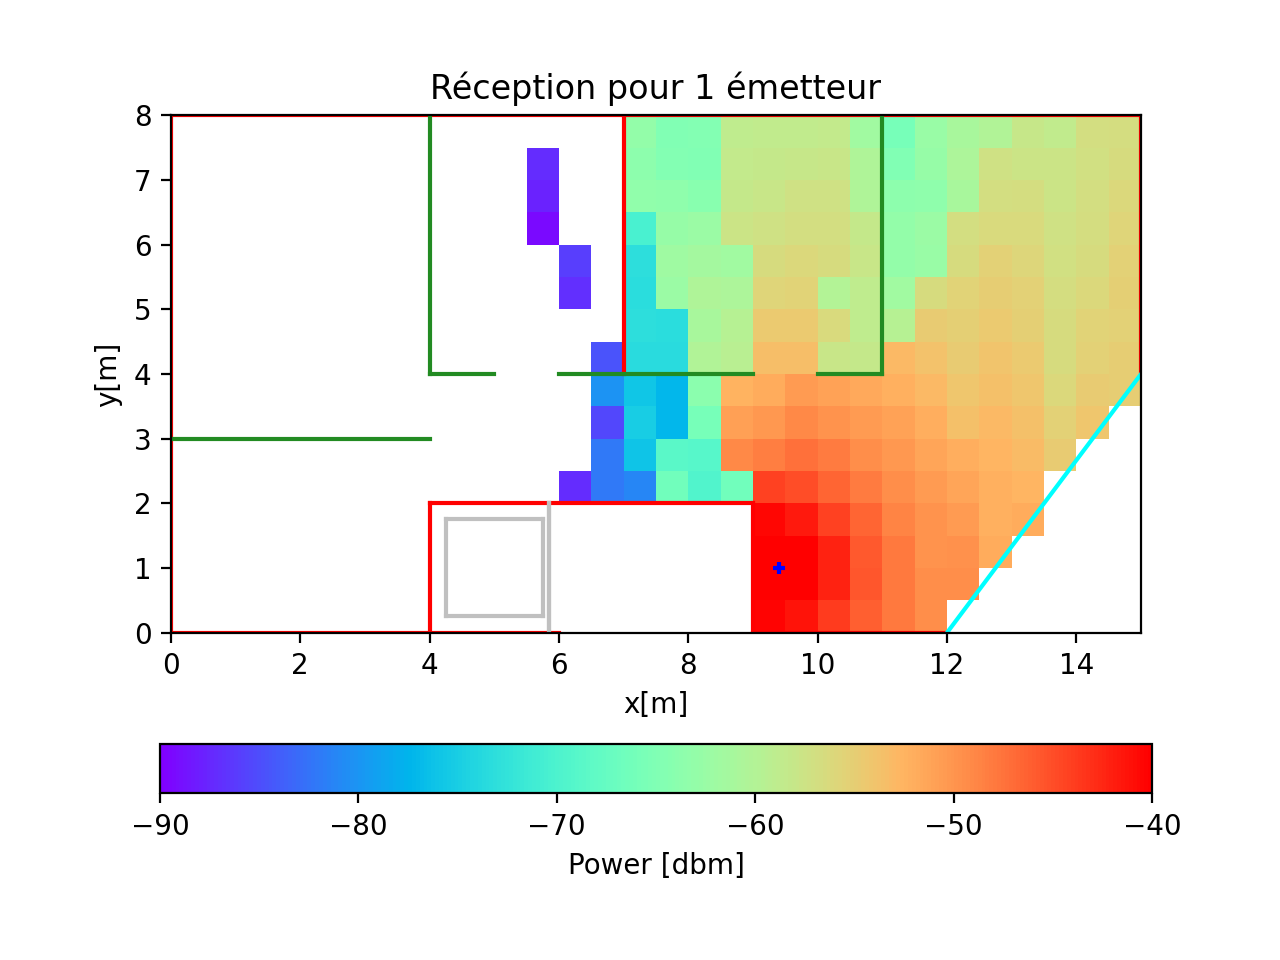
\includegraphics[width=0.6\textwidth]{images/verif/elevator.png}
    \caption{Émetteur dans la position suggérée : tx = (9.4, 1.0); grille de pas 0.5m, \textbf{avec ascenseur}}
    \label{fig:elevator}
    
\end{figure}

On constate aussi qu'un unique émetteur dans la position suggérée ne suffira pas à couvrir l'ensemble des bureaux.

\section{Suggestion pour améliorer la réception}

Le but est de trouver un compromis entre le nombre d'émetteurs (donc prix) et couverture\footnote{Le terme couverture traduit que l'on privilégie d'avoir une bonne reception partout plutôt qu'une excellente réception localisée}.

\subsection{Recherche de maximum}
Pour commencer, il faut savoir où placer ces émetteurs. pour cela,
nous allons utiliser un algorithme de recherche de maximum global.
Nous sommes ici en présence d'un problème peu continu car changer un peu 
la position d'un émetteur
peut d'un coup lui permettre d'atteindre une nouvelle piece.
Dans ce cadre peu continu, les algorithmes conventionnels purement déterministes
auront du mal à converger.

C'est pourquoi il a été nécessaire de prendre un algorithme avec une partie un peu
plus aléatoire, d'évolution générationnelle. Celle-ci à été mélangée
avec un algorithme de manipulation géométrique pour l'étape de mutation. Cet algorithme
est appelé \textbf{évolution différentielle}.

% \begin{tcolorbox}[colback=blue!10!white,colframe=blue!50!black,title=Evolution differentielle,sharp corners]
%     L'evolution différentielle mélange algorithme génétique et technique géométrique.
%     Nous avons une population d'individus dont les mutations et recombinaisons sont dictées 
%     par une manipulation géométrique.
% \end{tcolorbox}

Nous prenons l'implementation de la librairie \textit{scipy}

\texttt{scipy.optimize.differential\_evolution(func, bounds, args=(n), strategy='best1bin', popsize=40)}
\begin{itemize}
    \item \textbf{func} sera notre fonction coût (voir \ref{sub:arch_opti})
    \item \textbf{bounds} délimite la zone dans laquelle on peut placer nos émetteurs (ici : l'appartement) 
    \item \textbf{pop\_size} augmentera la population d'essais ce qui augmentera nos chances de tomber sur le maximum global.

\end{itemize}

\subsection{Architecture d'optimisation}
\label{sub:arch_opti}

Le plus important ici est de trouver une fonction coût pour emmener l'algorithme
vers la solution de manière rapide et fiable.
Ici nous prenons $f = \sqrt{\sum_{i,j}power[i,j]^2}$ (rms) que l'algorithme tentera de maximiser.
Prendre le carré des valeurs de puissance permet de punir d'avantage les endroits où
la reception est mauvaise et d'augmenter le gradient des valeurs de $f$ ce qui 
augmente la vitesse de convergence. 

Pour focaliser l'algorithme sur la maximisation de la couverture,
on ignore les valeurs de puissance au dessus de $-50dbm$ qui ne représentent que la puissance
à immédiate proximité de l'antenne. On peut effectivement voir sur la figure \ref{fig:coupure}
que cette restriction mène effectivement à une amélioration de la couverture globale.

\begin{figure}[H]
    \centering
    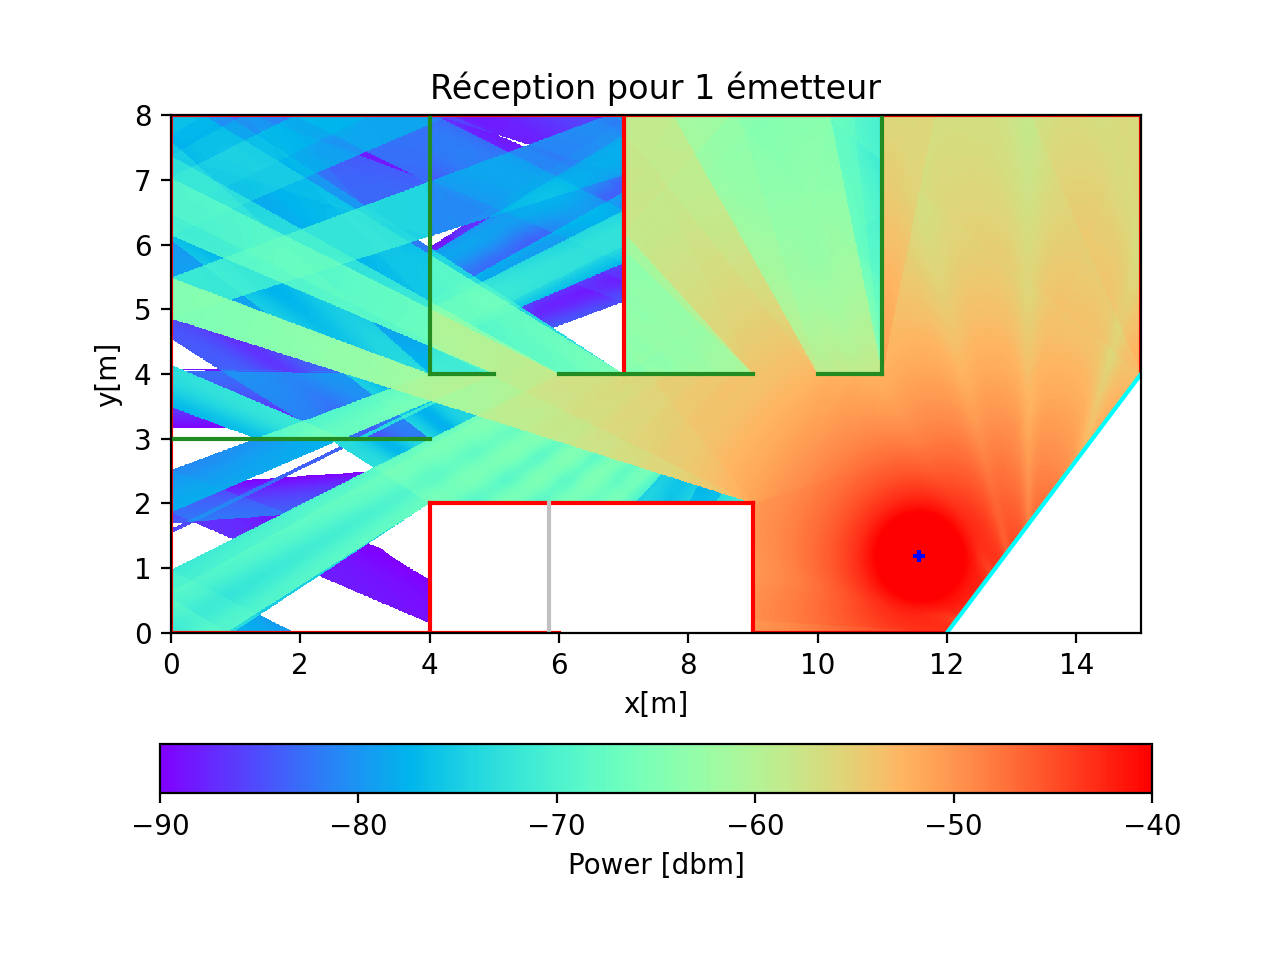
\includegraphics[width=0.49\textwidth]{images/optimize/1_dbm_40.png}
    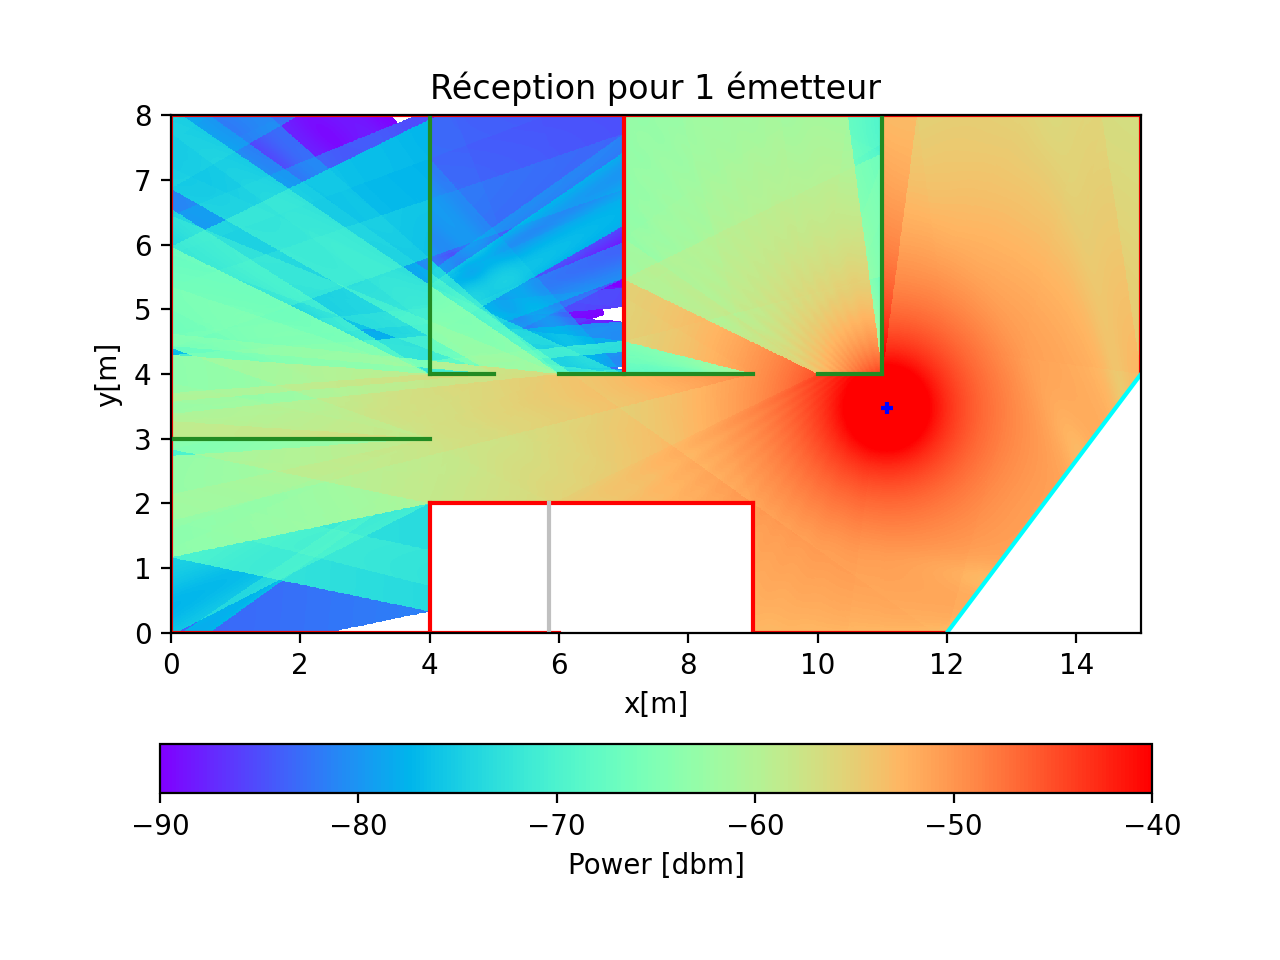
\includegraphics[width=0.49\textwidth]{images/optimize/1_dbm.png}
    \caption{A gauche : coupure à $-40dbm$; A droite : coupure à $-50dbm$}
    \label{fig:coupure}
\end{figure}


L'optimisation s'effectue sur une grille de pas $0.2m$. Les coordonnées optimales
trouvées sont ensuite affichées avec une grille de pas $0.05m$

L'algorithme a eu tendance à placer l'antenne pile dans un mur, ce qui empêchait la détection
de la transmission et donc de l'atténuation en résultant. Il a donc fallu ajouter une condition
pour éviter cet endroit.





\subsection{Essais d'optimisation}

Essayons avec un émetteur.

\begin{figure}[H]
    \centering
    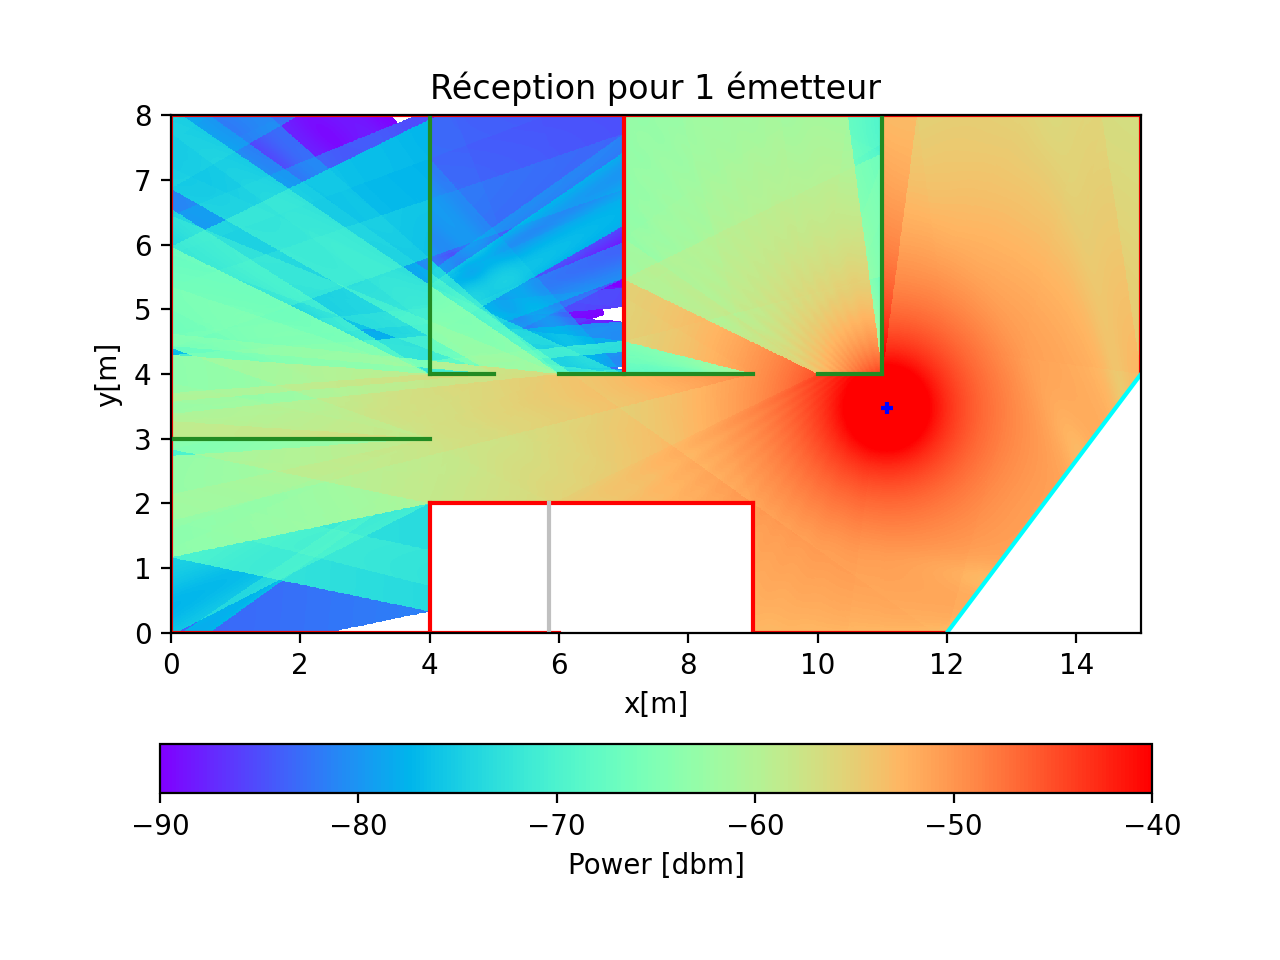
\includegraphics[width=0.6\textwidth]{images/optimize/1_dbm.png}
    % 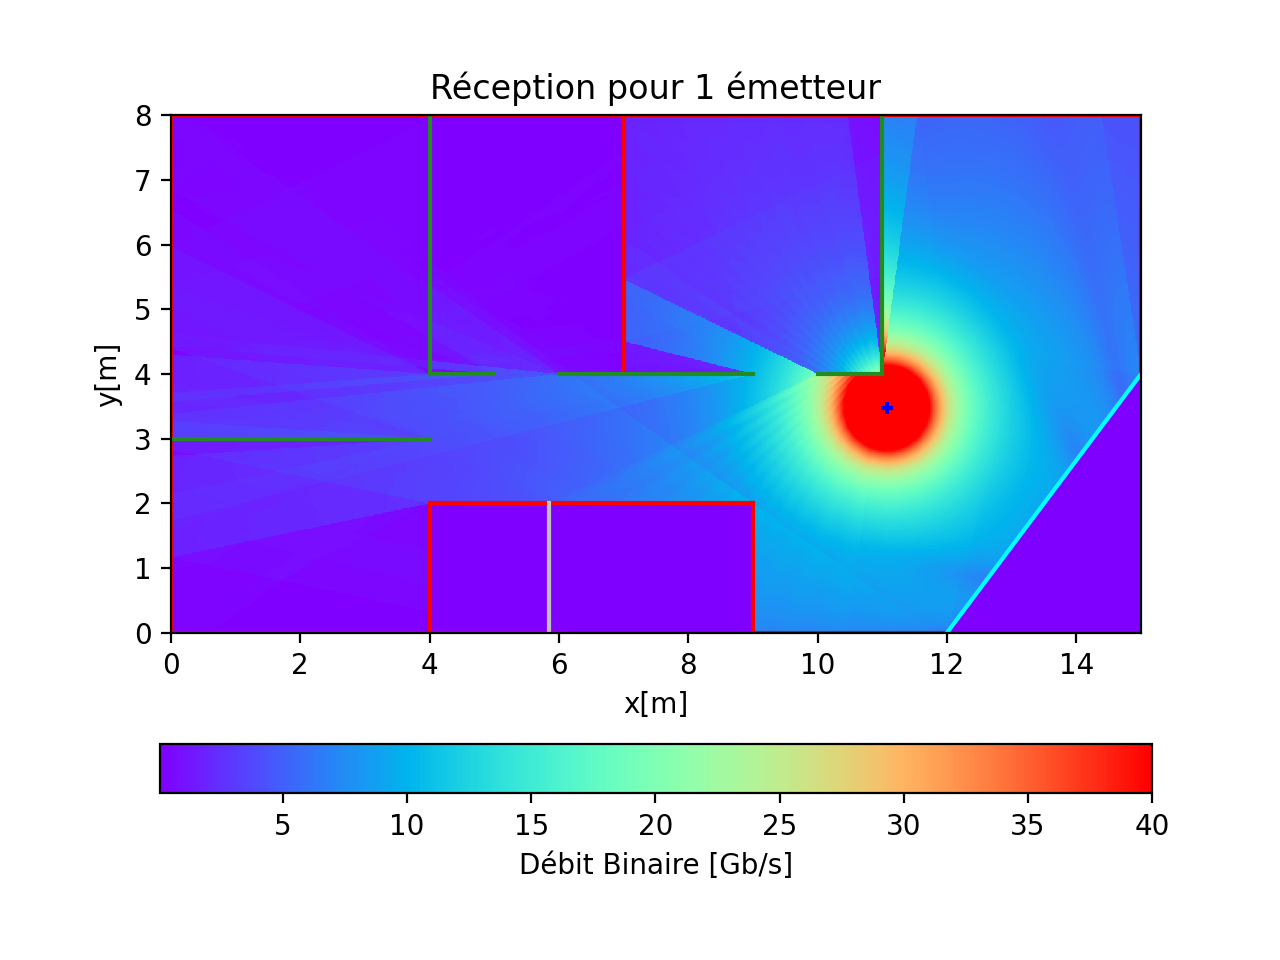
\includegraphics[width=0.49\textwidth]{images/optimize/1_bin.png}
\end{figure}

On voit que cet emplacement offre une meilleure couverture mais que ça reste insuffisant pour
couvrir l'ensemble de l'espace correctement. 

En réalité, on peut placer un émetteur plus au milieu de 
l'appartement et obtenir une meilleure couverture mais avec 
avec une puissance totale (sans coupure à -50dbm) et rms sensiblement plus faible.
Dans nos critères, couper à -50dbm est très arbitraire et pourrait être
adapté en fonction du nombre d'émetteurs et donc
la puissance qu'on pourrait espérer avoir globalement mais c'est une valeur
qui fonctionne bien lorsque l'on cherche à assurer un débit de l'ordre de 10Gb/s.

Regardons ce qui se passe quand on ajoute un 2ème émetteur.

\begin{figure}[H]
    \centering
    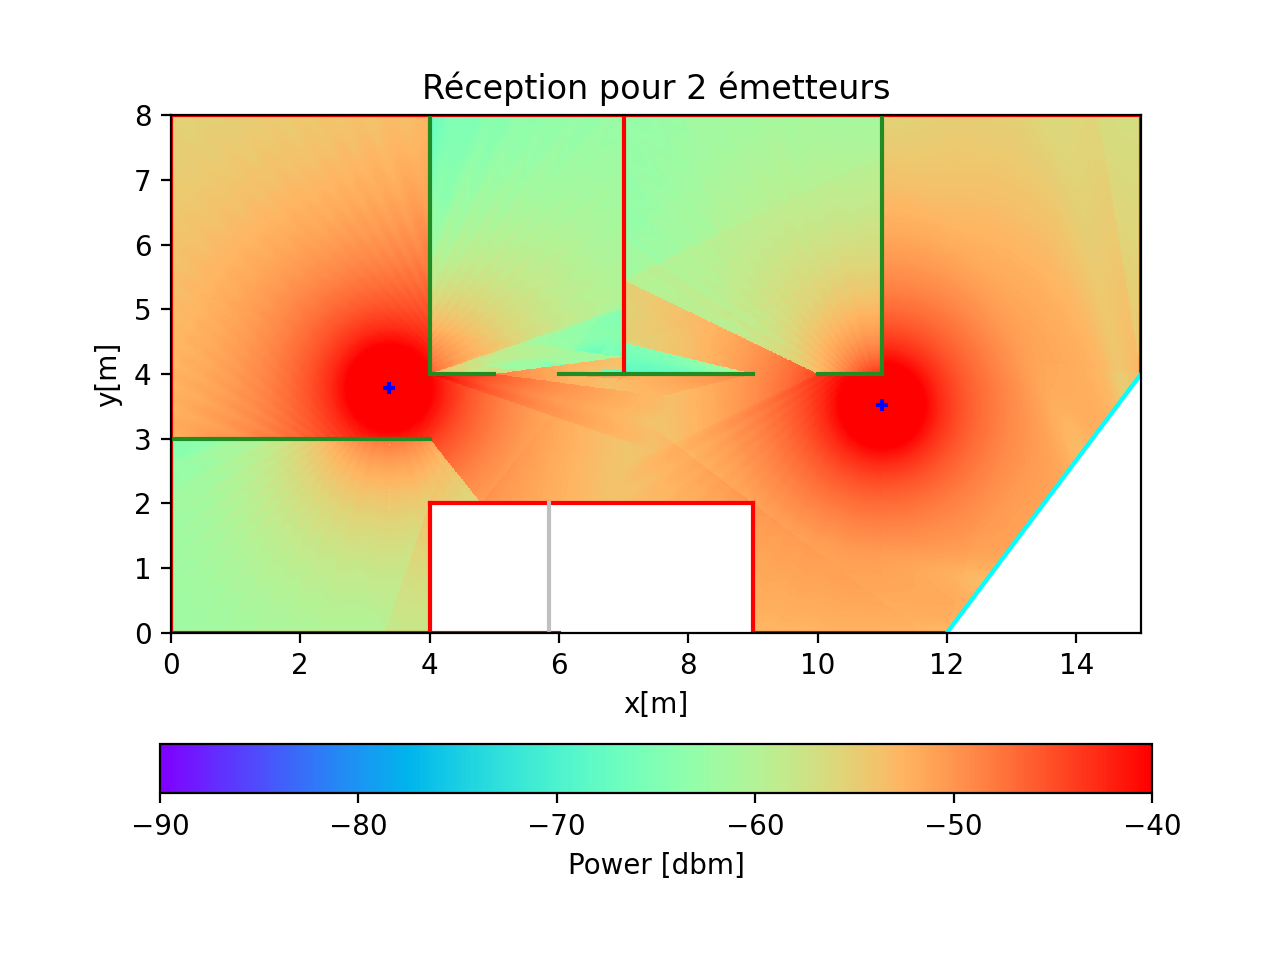
\includegraphics[width=0.6\textwidth]{images/optimize/2_dbm.png}
    % 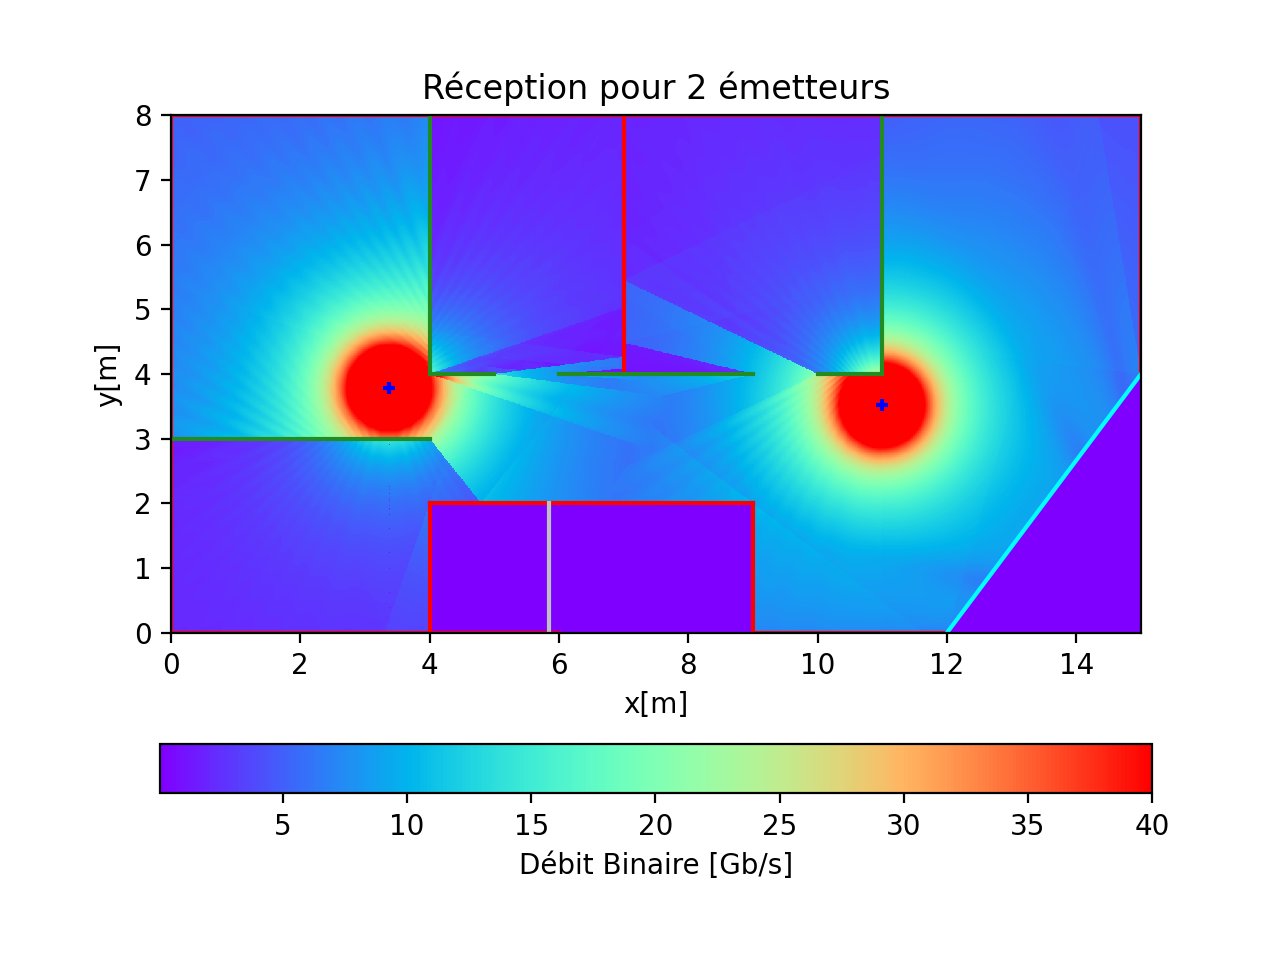
\includegraphics[width=0.49\textwidth]{images/optimize/2_bin.png}
\end{figure}

On parvient à rester $\ge -65db$ partout ce qui équivaut à $1.4 Gb/s$.

Des exemples avec plus d'émetteurs sont dans les sous annexes de \ref{sub:more_emit}.
Ils seront discutés plus tard.

\subsection{Conclusion sur le nombre d'émetteurs}
Plutôt que de montrer à chaque fois la répartition, regardons des variables
plus globales.

\begin{figure}[H]
    \centering
    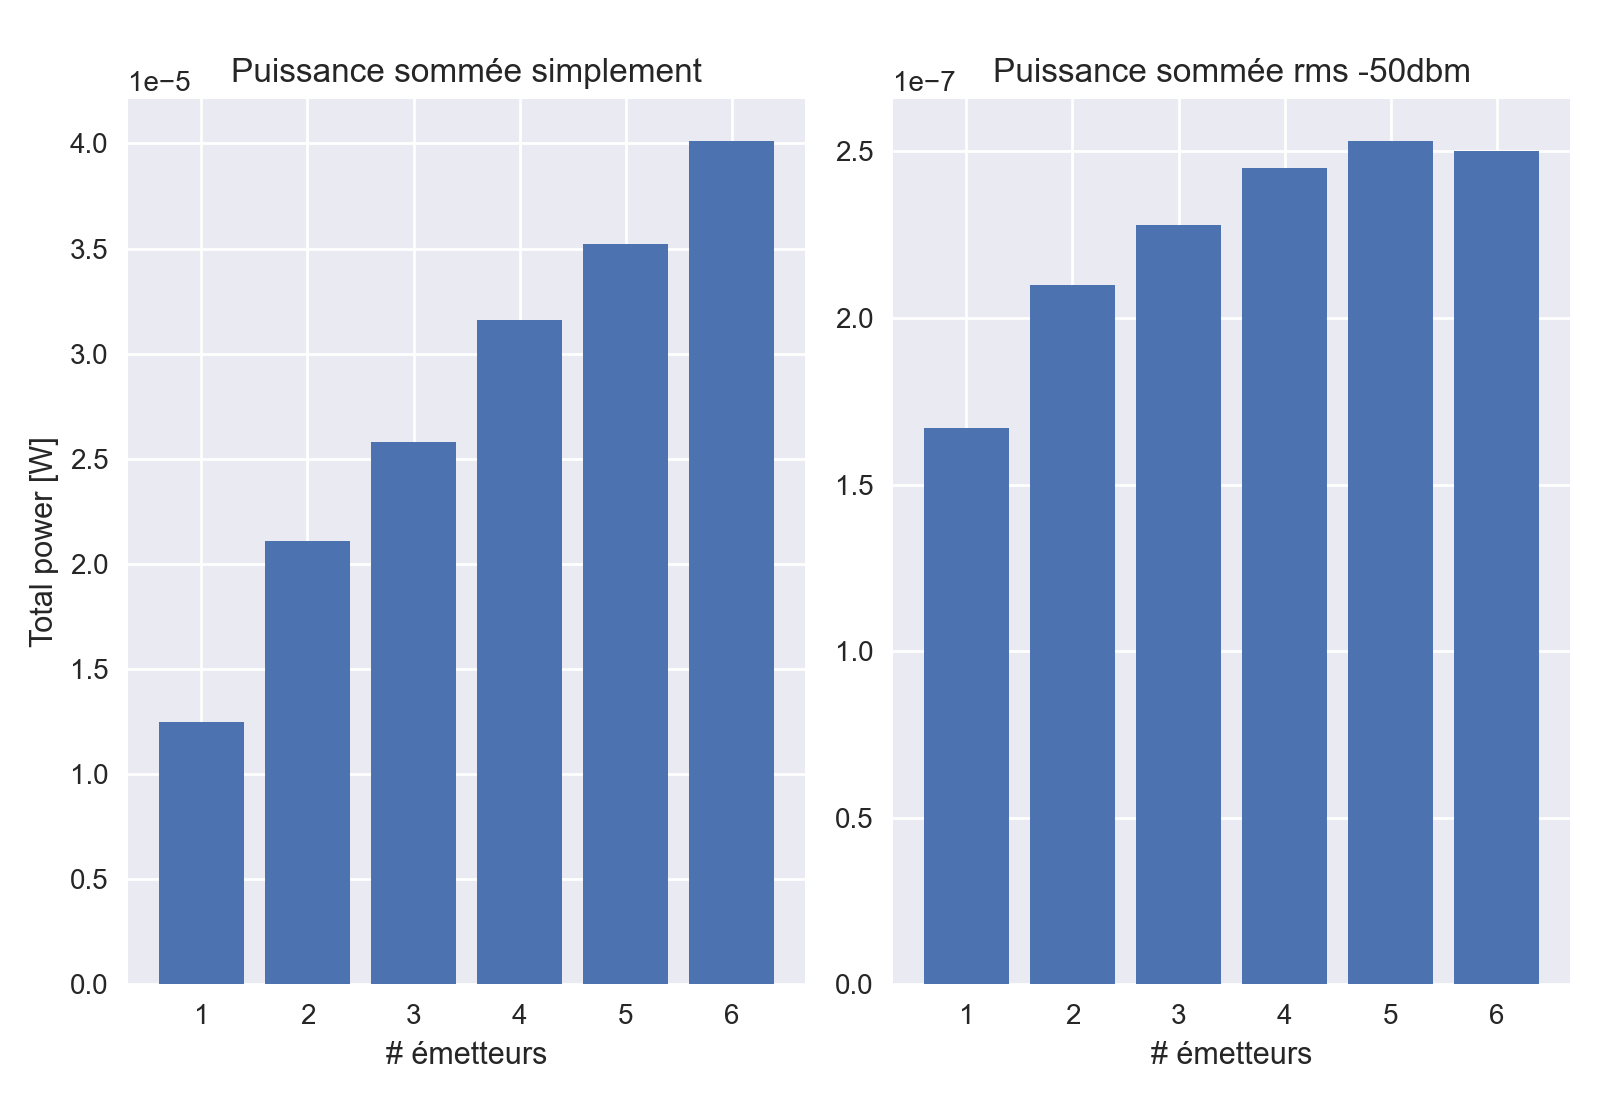
\includegraphics[width=0.8\textwidth]{images/optimize/data_compare.png}
    \caption{Evolution de la puissance totale et de la couverture}
    \label{fig:datacomp}
\end{figure}

Attention, sur la figure \ref{fig:datacomp} les fonctions coût sont différentes. 
\begin{itemize}
    \item A gauche: on effectue une somme simple, non bornée aux valeurs $< -50dbm$ mais plutôt à $< -40dbm$
    Ce qui donne une somme exacte de la puissance reçue.
    
    \item A droite: on utilise la fonction coût rms de \ref{sub:arch_opti} avec cette restriction
    aux valeurs $< -50dbm$ qui traduira donc mieux la qualité de la couverture.
\end{itemize}

A gauche,
la fonction coût est une simple sommation des puissances, à droite,
on a la fonction coût comme décrite avant en \textit{rms}.


% \begin{tcolorbox}[colback=blue!10!white,colframe=blue!50!black,title=Conclusion,sharp corners]
La figure \ref{fig:datacomp} montre que placer 2 émetteurs
est un minimum et qu'on atteint une presque saturation à partir de 4 du critère de couverture rms 
qui s'explique par le plafond à -50dbm dans la sommation.
Cette saturation traduit bien que au delà de 4 émetteurs, la couverture à plus de -50dbm ($\sim 10Gb/s$) est
assurée presque partout.

La solution à 4 émetteurs ne permet pas de couvrir parfaitement
une des pièces (voir \ref{sub-4}). Celle-ci étant
relativement petite, elle pourrait servir de salle à machines à cafés
qui ne requiert par la meilleure réception.

Si la couverture parfaite de tout l'étage est requise, 
Il suffit de passer à la solution à 5 émetteurs (voir \ref{sub-5})

% \end{tcolorbox}


\section{Annexes}

% \subsection{Données du problème du Syllabus}
% \begin{itemize}
%     \item $f = 868.3 \times 10^6$, $\omega = 2\pi f$, $\lambda = \frac{c}{f}$
%     \item $\beta = \omega \sqrt{\mu_0  \epsilon_0}$
%     \item $\epsilon_r = 4.8$
%     \item $\sigma = 0.018 S/m$
%     \item $l = 0.15m$
%     \item $Z_0 = 120\pi$
%     \item $R_{ar} = 73 \Omega$
%     \item $P_{tx} = 10^{-3} W$
% \end{itemize}

\subsection{Plus d'émetteurs}\label{sub:more_emit}
\subsubsection{Trois émetteurs}
\label{sub-3}

\begin{figure}[H]
    \centering
    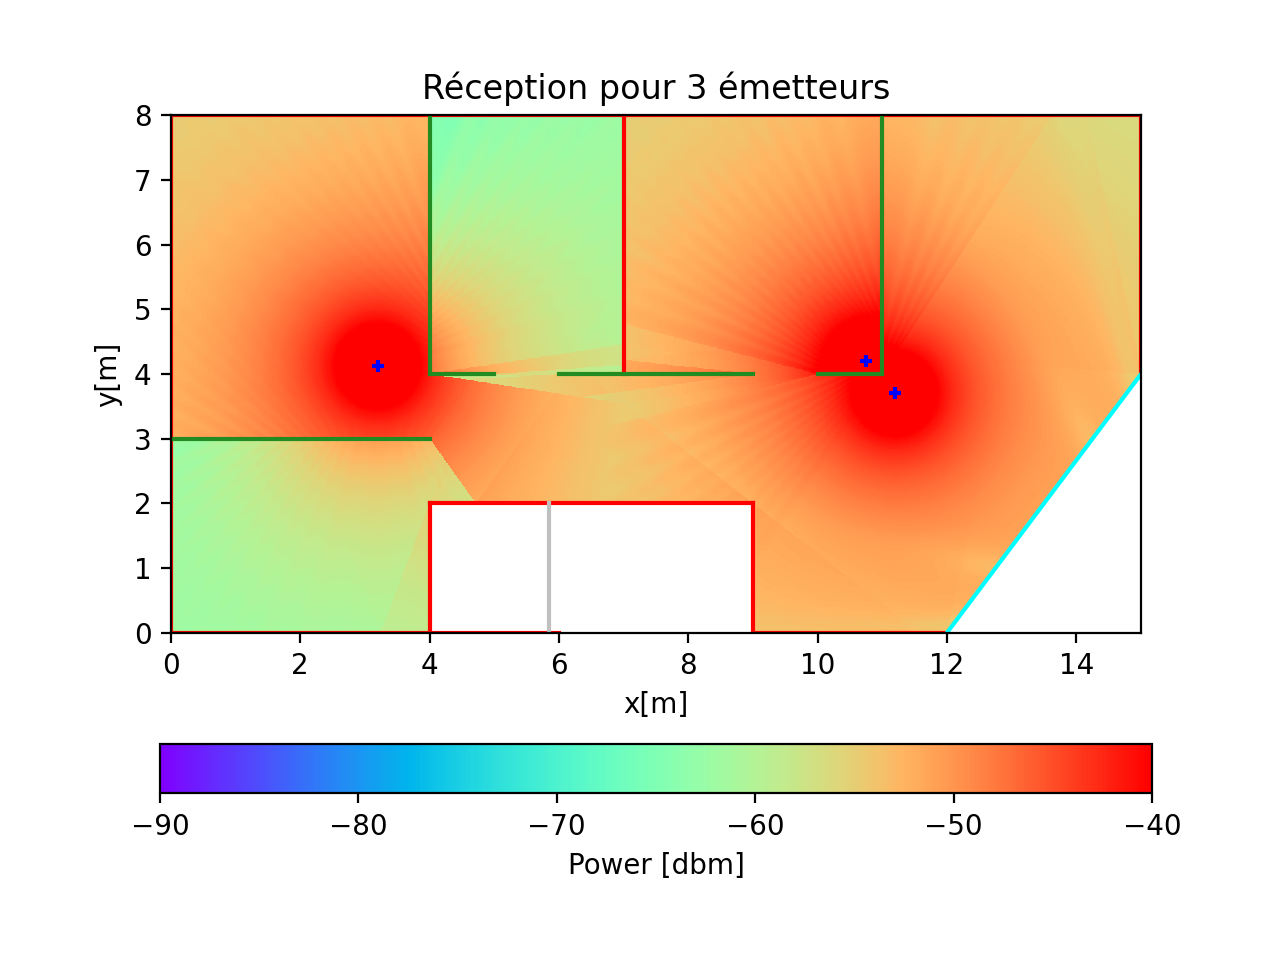
\includegraphics[width=0.6\textwidth]{images/optimize/3_dbm.png}
    % 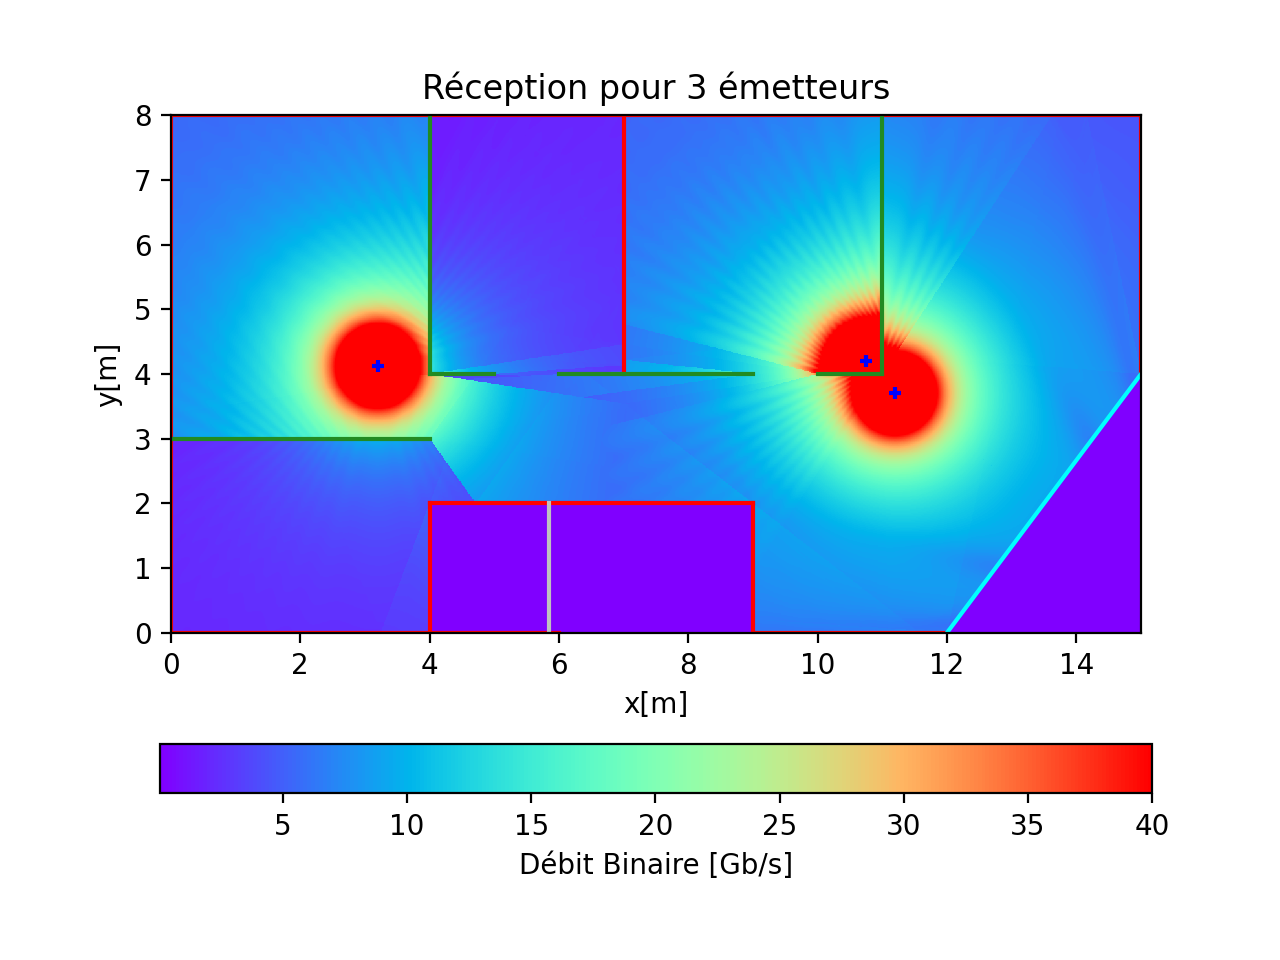
\includegraphics[width=0.49\textwidth]{images/optimize/3_bin.png}
\end{figure}

\subsubsection{Quatre émetteurs}
\label{sub-4}

\begin{figure}[H]
    \centering
    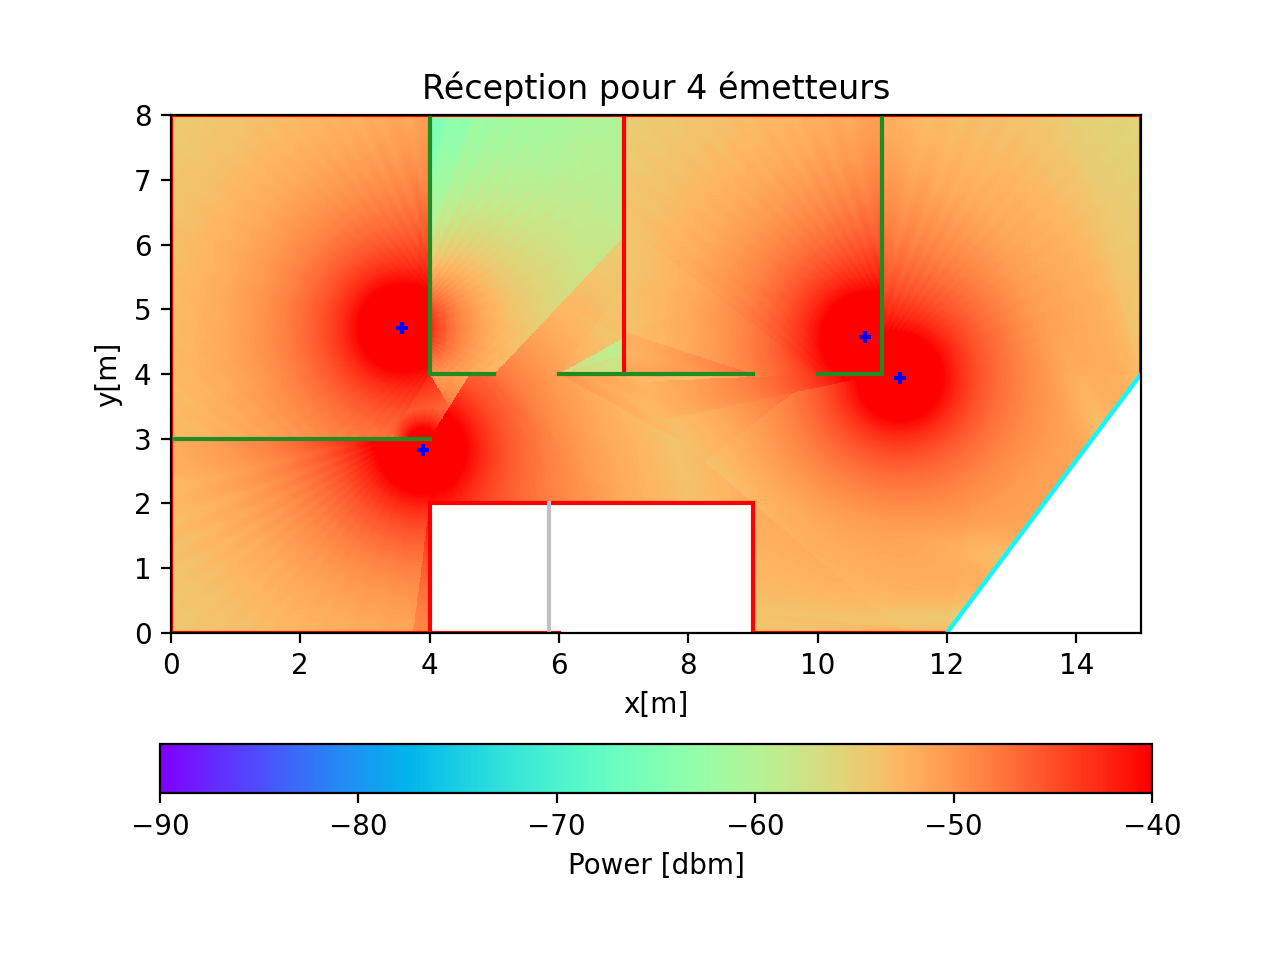
\includegraphics[width=0.6\textwidth]{images/optimize/4_dbm.png}
    % 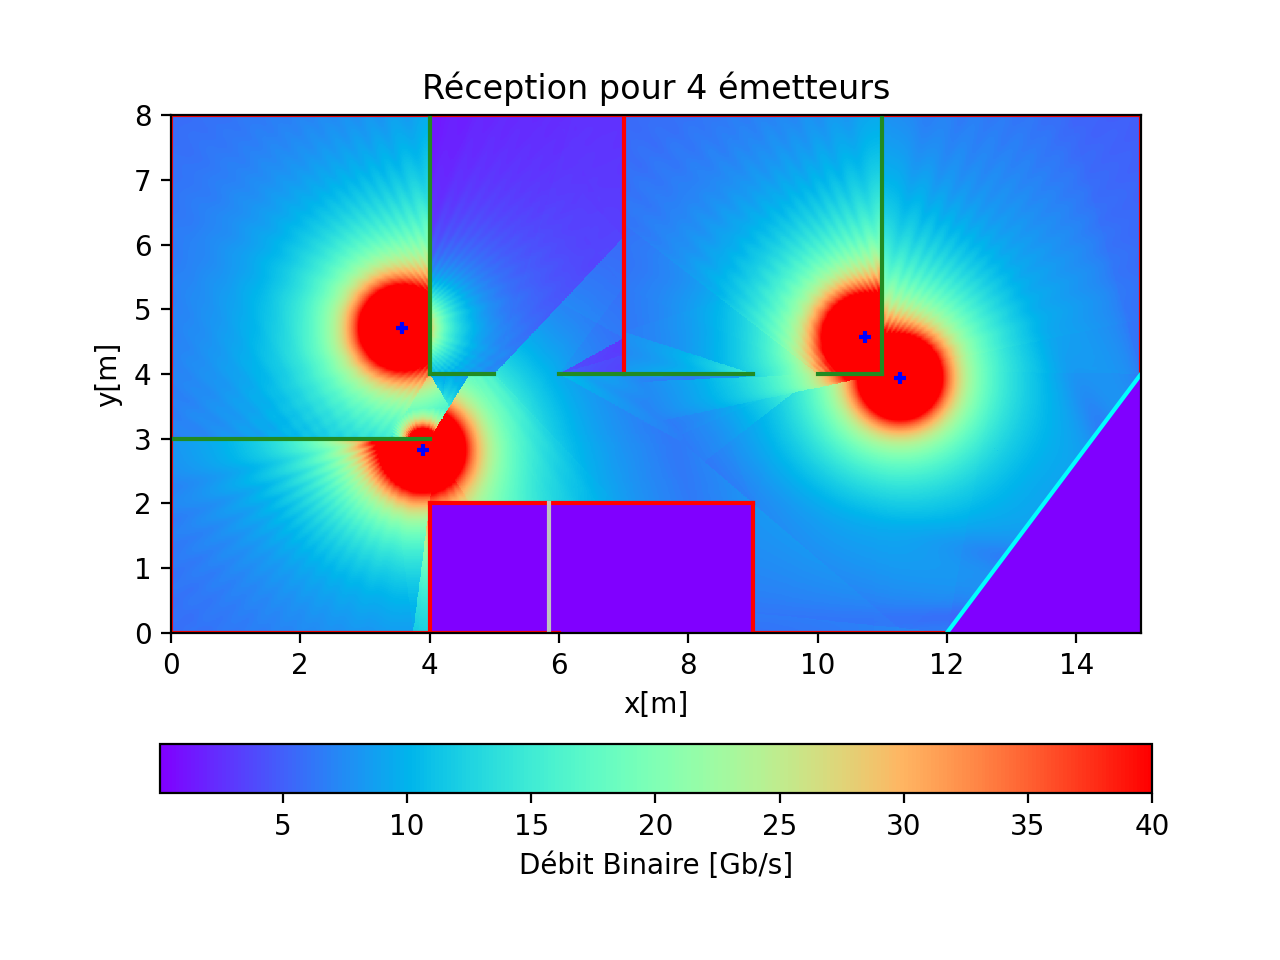
\includegraphics[width=0.49\textwidth]{images/optimize/4_bin.png}
\end{figure}

\subsubsection{Cinq émetteurs}
\label{sub-5}

\begin{figure}[H]
    \centering
    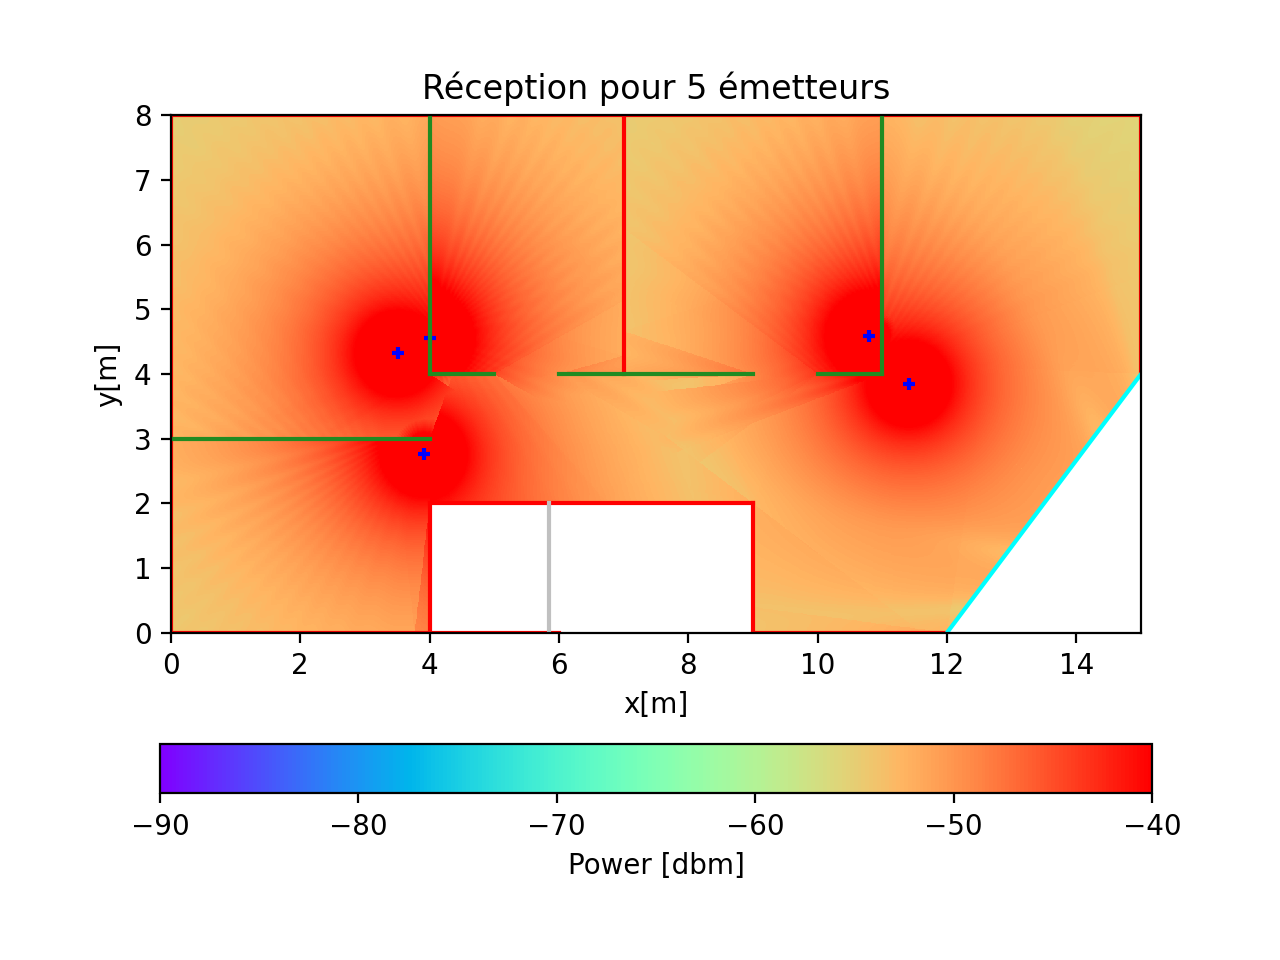
\includegraphics[width=0.6\textwidth]{images/optimize/5_dbm.png}
    % 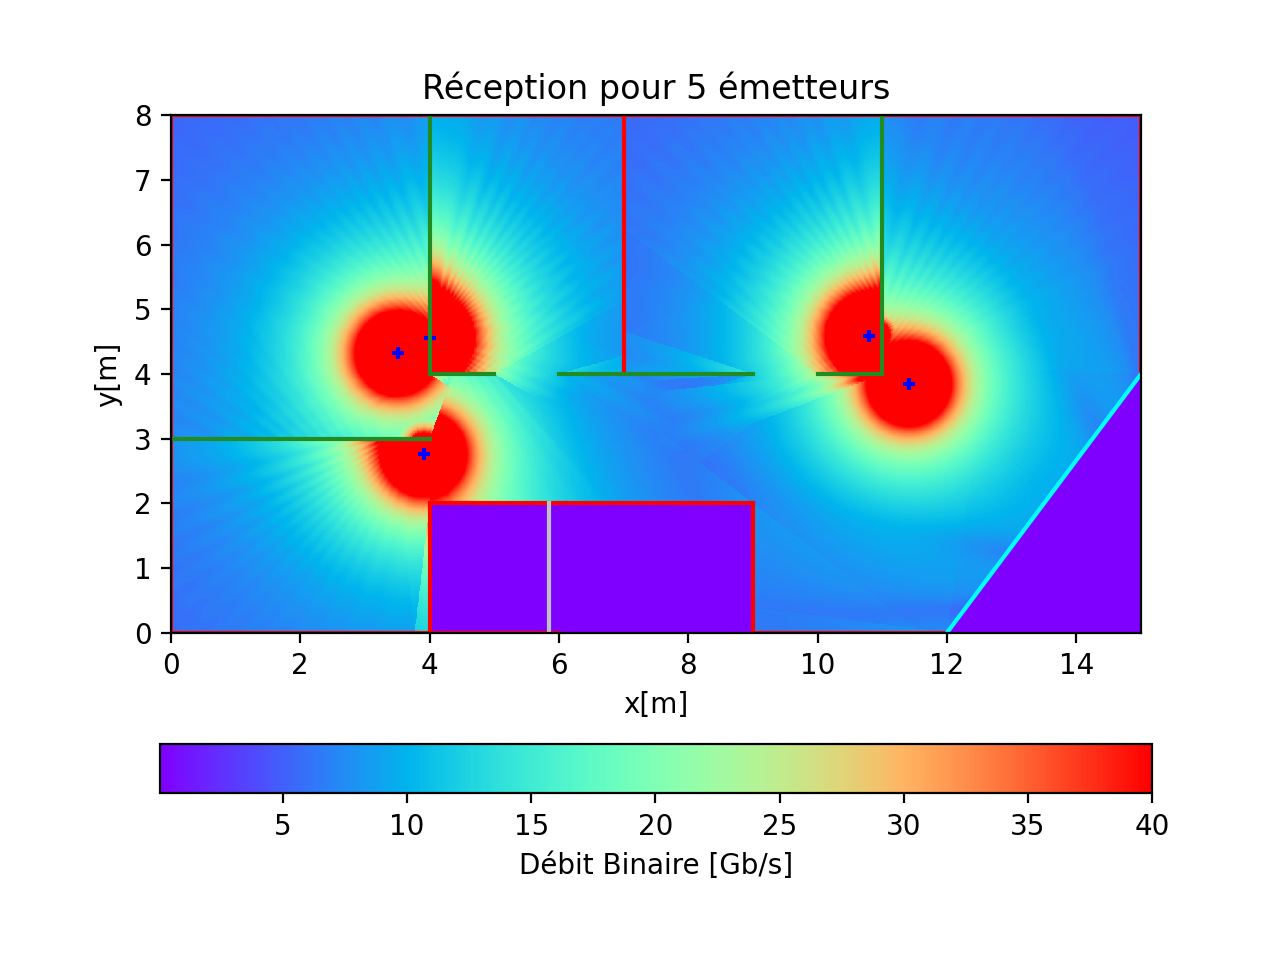
\includegraphics[width=0.49\textwidth]{images/optimize/5_bin.png}
\end{figure}

A partir de 5 émetteurs, le temps de calcul devient vraiment long,
pour une \texttt{pop\_size = 40} l'algorithme fait appel $212811$ fois à la 
fonction \texttt{get\_power()}

\subsubsection{Six émetteurs}
\label{sub-6}

\begin{figure}[H]
    \centering
    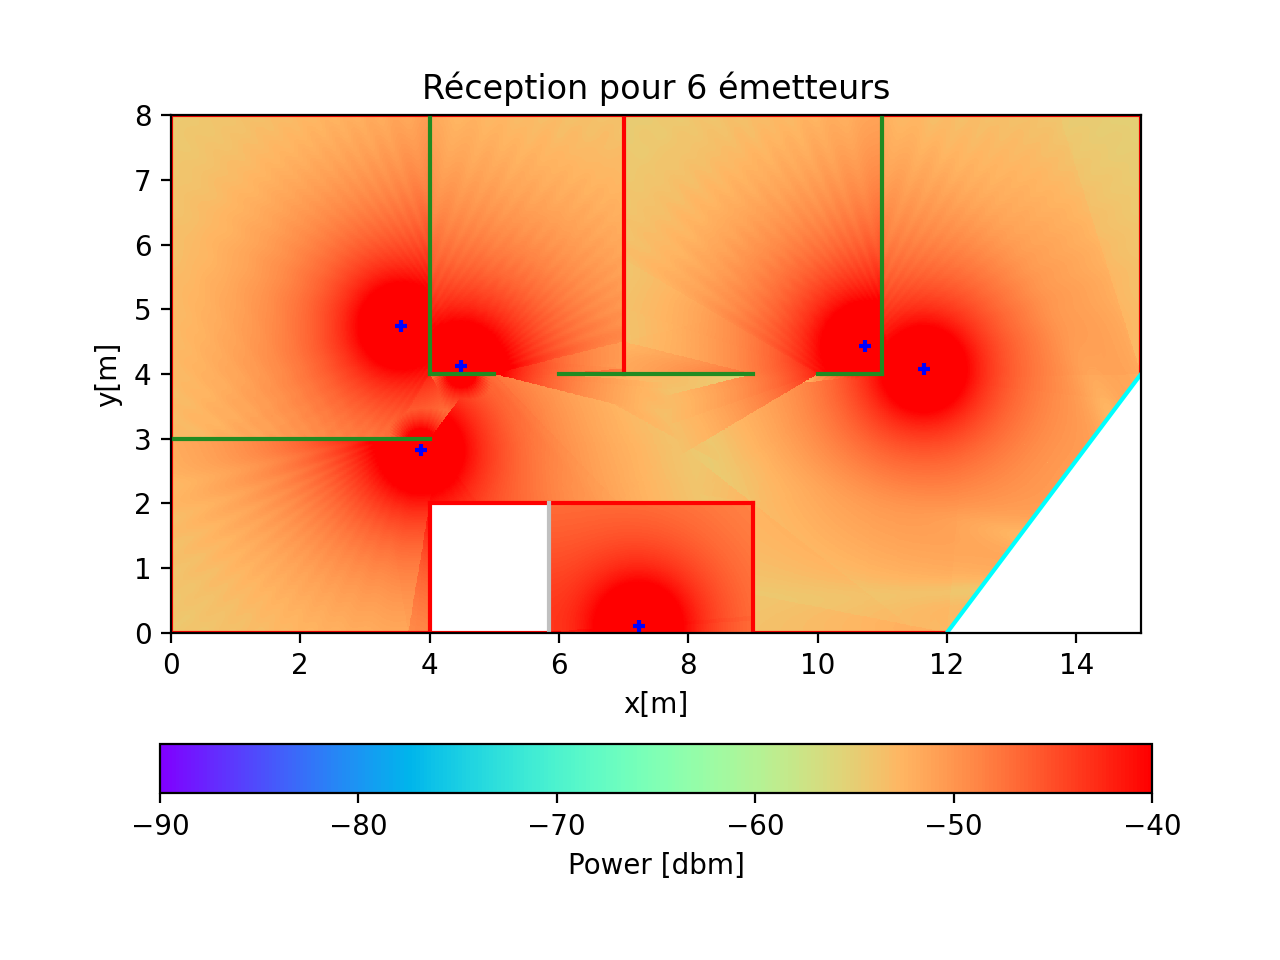
\includegraphics[width=0.49\textwidth]{images/optimize/6_dbm.png}
    % 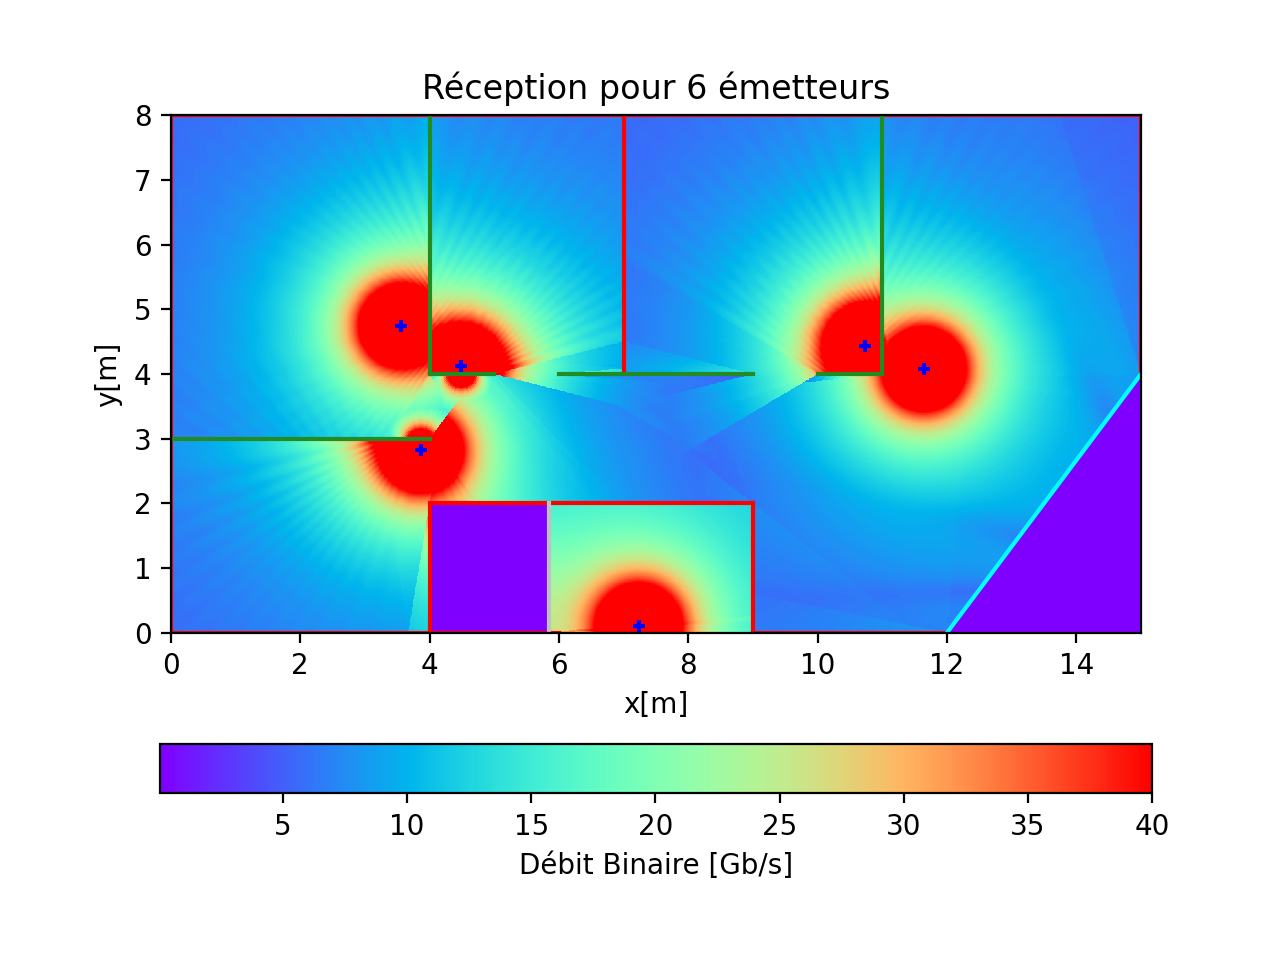
\includegraphics[width=0.49\textwidth]{images/optimize/6_bin.png}
\end{figure}

Avec 6 émetteurs on commence à remplir des espaces inutiles comme la zone de l'ascenseur.

\subsection{Code}

\subsubsection{Main}

\begin{lstlisting}[language=python]
from world import world
from grid_solver import *
from display import image
from optimizer import *
from data import *
from rays import *

""" Allocating and transferring gpu memory for walls """
world.allocate()
world.transfer()

""" Optimisation """
grid = Grid(n)
grid.generate_grid()
result = txs_optimize(grid)
print(result)  # contains information like number of iteration, optimal position and cost function value
print("rms : ", grid.get_rms())
print("total : ", grid.get_total())

""" Use the optimized positions and
display it with a better resolution """
del grid  # freeing old data
dim.update(0.5)  # updating the resolution
precise_grid = Grid(n)
precise_grid.generate_grid()
txs = result.x.astype(np.float32)  # to use the optimized txs
# txs = tx.to_numpy()  # to use the tx defined in data
precise_grid.fill_power(txs)
precise_grid.power_to_dbm()  # fills array of dbm
precise_grid.dbm_to_binary()  # fills array of binary debit

""" Rays """
# rays.init_after_world(world, tx, rx)
# test_rays(rays)

""" Extract images """
image.re_init()
# image.draw_rays(rays)
image.plot_function(precise_grid.rx_powers_dbm.to_numpy(), "dbm")
image.plot_emitters(txs)
image.show()
image.extract(f"./exports/{n}_dbm.png")
image.re_init()
image.plot_function(precise_grid.rx_binary.to_numpy(), "binary")
image.plot_emitters(txs)
image.show()
image.extract(f"./exports/{n}_bin.png")

\end{lstlisting}

\subsubsection{Grid Solver}

\begin{lstlisting}[language=python]
from utils import *
from data import *
from unit_solver import calculate_power
from world import world


@ti.data_oriented
class Grid:
    def __init__(self, n):
        self.rx_centers = ti.Vector.field(2, dtype=ti.f32)
        self.rx_powers_n = ti.field(ti.f32)
        self.rx_powers = ti.field(ti.f32)  # where the best from rx_powers_n is extracted
        self.rx_powers_dbm = ti.field(ti.f32)  # converted to dbm
        self.rx_binary = ti.field(ti.f32)  # converted to binary debit
        self.n = n  # number of emitters
        ti.root.dense(ti.ijk, (dim.y, dim.x, n)).place(self.rx_powers_n)
        ti.root.dense(ti.ij, (dim.y, dim.x)).place(self.rx_centers)
        ti.root.dense(ti.ij, (dim.y, dim.x)).place(self.rx_powers, self.rx_powers_dbm, self.rx_binary)  # AoS

    @ti.kernel
    def generate_grid(self) -> ti.i32:
        # fills the rx_centers array with all rx coordinate with respect to cell size
        for i, j in self.rx_centers:
            x = dim.cell_size / 2.0 + j * dim.cell_size
            y = dim.cell_size / 2.0 + i * dim.cell_size
            self.rx_centers[i, j] = vec2([x, y])
        return 0

    @ti.kernel
    def fill_power(self, txs: ti.types.ndarray(dtype=ti.f32, ndim=1)):
        # accepting numpy array as pos makes the code slower here
        # but since the optimization algorithm sends numpy arrays of positions
        # this is still faster compared to manual conversion
        for i, j, k in self.rx_powers_n:
            # i,j are all the grid receiver points
            # k is the chosen emitter in the n sized array
            if self.rx_centers[i, j][0] >= 12.0 and self.rx_centers[i, j][1] <= (4.0 / 3.0 * (self.rx_centers[i, j][0] - 12.0)):
                # avoids unwanted area behind the glass panel
                self.rx_powers_n[i, j, k] = 0.0
            else:
                self.rx_powers_n[i, j, k] = PRX0 * calculate_power(world, vec2([txs[2*k], txs[2*k+1]]), self.rx_centers[i, j])

        for i, j in self.rx_powers:
            # we have the results for all emitters, now we need to take the best ones
            current_best = ti.f32(0.0)
            # serialized
            for k in range(self.n):
                if self.rx_powers_n[i, j, k] > current_best:
                    current_best = self.rx_powers_n[i, j, k]
            self.rx_powers[i, j] = current_best

    @ti.kernel
    def power_to_dbm(self):
        for i, j in self.rx_powers_dbm:
            power = ti.f32(10.0) * log10(self.rx_powers[i, j] * 1e3)
            if power < -90.0:
                # under -90dbm, the receiver cannot process the signal
                # therefore, we cut it there and place -inf dbm instead, equivalent
                # to a power of 0
                power = -tm.inf
            elif power > -40.0:
                # the receiver is limited to a reception of -40 dbm signal
                power = -40.0
            self.rx_powers_dbm[i, j] = power

    @ti.kernel
    def dbm_to_binary(self):
        # translates the linear relationship of dbm to log(binary)
        # and then converts it back to binary in GHz
        for i, j in self.rx_binary:
            dbm = self.rx_powers_dbm[i, j]
            if -90 <= dbm <= -40:
                bd_log = 6 + log10(50) + ((3 + log10(40) - log10(50))/50 * (dbm + 90))
                bd = 10**bd_log * 1e-9
                self.rx_binary[i, j] = bd

    @ti.kernel
    def get_rms(self) -> ti.f32:
        # used in the cost function
        rms = 0.0
        # parallelized
        for j in range(dim.x):
            sub_total = 0.0
            # serialized
            for i in range(dim.y):
                elem = self.rx_powers[i, j]
                if elem >= P_MAX_50 or elem <= P_MIN:
                    continue
                else:
                    sub_total = sub_total + ti.pow(elem, 2)
            # has to be explicitly atomic
            ti.atomic_add(rms, sub_total)
        return ti.sqrt(rms)

    @ti.kernel
    def get_total(self) -> ti.f32:
        total = 0.0
        # parallelized
        for j in range(dim.x):
            sub_total = 0.0
            # serialized
            for i in range(dim.y):
                elem = self.rx_powers[i, j]
                if elem >= P_MAX_40 or elem <= P_MIN:
                    continue
                else:
                    sub_total = sub_total + elem
            # has to be explicitly atomic
            ti.atomic_add(total, sub_total)
        return total

\end{lstlisting}

\subsubsection{Optimizer}

\begin{lstlisting}[language=python]
from grid_solver import *
from scipy.optimize import Bounds
from scipy.optimize import differential_evolution, direct, dual_annealing, shgo


def txs_cost_function(pos, grid):
    for i in range(n):
        if 0.0 <= pos[2*i] <= 5.0 and 2.90 <= pos[2*i+1] <= 3.10:
            # to prevent the algorithm from placing the emitter inside this wall
            return 0.0
    grid.fill_power(pos.astype(np.float32))
    return -grid.get_rms()


def get_bounds(n):
    # filling bounds within where the algorithm can place emitters
    bottom_left = [0.0 for _ in range(2*n)]
    upper_right = []
    for _ in range(n):
        upper_right.append(15.0)
        upper_right.append(8.0)
    return Bounds(bottom_left, upper_right)


@measure_execution_time
def txs_optimize(grid):
    bounds = get_bounds(grid.n)
    result = differential_evolution(txs_cost_function, bounds, args=[grid], strategy='best1bin', popsize=40)
    return result

\end{lstlisting}

\subsubsection{Unit Solver}

\begin{lstlisting}[language=python]
from utils import *
from wall import Wall  # importing static methods for coefficients calculation
from data import P_MAX_CL


@ti.func
def intersect(u, n, p1, q1, p2, q2):
    # checks if there is an intersection between wall (u,n,p1,q1)
    # and a ray (p2, q2)
    value = False
    if tm.sign((q2 - p1).dot(n)) != tm.sign((p2 - p1).dot(n)):
        t = find_intersection(p1, u, p2, q2)
        ip = Wall.point_on_wall(p1, u, t)
        if tm.sign((ip - p1).dot(u)) != tm.sign((ip - q1).dot(u)):
            value = True
    return value


@ti.func
def dist(r0, u, p):
    return ti.abs(u[1] * p[0] - u[0] * p[1] - u[1] * r0[0] + u[0] * r0[1])


@ti.func
def get_next_tx(r0, u, n, tx):
    # gets the symmetric of tx by the wall plane (r0, u, n)
    return tx - 2 * n * tm.sign((tx - r0).dot(n)) * dist(r0, u, tx)


@ti.func
def find_intersection(r0, u, p2, q2):
    # this finds t, which will give the intersection point of the ray p2,q2
    # and the wall (r0,u) by intersection = t * u
    l = q2 - p2
    dx = l[0]
    dy = l[1]
    t = (dy * (r0[0] - q2[0]) - dx * (r0[1] - q2[1])) / (dx * u[1] - dy * u[0])
    return t


@ti.func
def bounce_cond(r0, n, p2, q2):
    # basic condition to know if the bounce is physically possible
    return tm.sign(n.dot(p2 - r0)) == tm.sign(n.dot(q2 - r0))


@ti.func
def wall_transmission(world, p2, q2, index1=-1, index2=-1):
    # see which walls are in the way of the ray defined by p2, q2
    # and calculates the total transmission coefficient for this ray
    # index1, index2 are walls that we don't want to take into account
    if index1 > index2:
        index_temp = index1
        index1 = index2
        index2 = index_temp

    transmission_factor_msq = ti.f32(1.0)
    ray_normal = (q2 - p2).normalized()
    for i in range(0, index1):
        p1, q1 = world.r0[i], world.r1[i]
        u, n = world.u[i], world.n[i]
        if intersect(u, n, p1, q1, p2, q2):
            transmission_factor_msq *= Wall.get_tn2(world, i, ray_normal)
    for i in range(index1 + 1, index2):
        p1, q1 = world.r0[i], world.r1[i]
        u, n = world.u[i], world.n[i]
        if intersect(u, n, p1, q1, p2, q2):
            transmission_factor_msq *= Wall.get_tn2(world, i, ray_normal)
    for i in range(index2 + 1, world.m):
        p1, q1 = world.r0[i], world.r1[i]
        u, n = world.u[i], world.n[i]
        if intersect(u, n, p1, q1, p2, q2):
            transmission_factor_msq *= Wall.get_tn2(world, i, ray_normal)
    return transmission_factor_msq


@ti.func
def calculate_power(world, tx, rx):
    # we avoid the problem of not being in "distant fields" hypothesis
    # by limiting the power value to its base value at a distance of 1m
    prx_temp = tm.clamp(1.0 / (tm.pow((rx - tx).norm(), 2)), 0.0, P_MAX_CL)

    trans0_0 = wall_transmission(world, rx, tx)
    prx = prx_temp * trans0_0

    for i in range(world.m):
        transmission_factor_msq = ti.f32(1.0)
        reflexion_factor_msq = ti.f32(1.0)
        r0_i, r1_i = world.r0[i], world.r1[i]
        u_i, n_i = world.u[i], world.n[i]
        tx1 = get_next_tx(r0_i, u_i, n_i, tx)
        if bounce_cond(r0_i, n_i, tx, rx):
            t = find_intersection(r0_i, u_i, tx1, rx)
            ip = Wall.point_on_wall(r0_i, u_i, t)
            if tm.sign((ip - r0_i).dot(u_i)) != tm.sign((ip - r1_i).dot(u_i)):
                reflexion_factor_msq *= Wall.get_rn2(world, i, (ip - tx).normalized())
                transmission_factor_msq *= wall_transmission(world, tx, ip, i) \
                                           * wall_transmission(world, ip, rx, i)
                prx_temp = tm.clamp(1.0 / ((rx - tx1).norm() ** 2), 0.0, P_MAX_CL)
                prx += prx_temp * transmission_factor_msq * reflexion_factor_msq

        for j in range(world.m):
            if i == j:
                continue
            transmission_factor_msq = ti.f32(1.0)
            reflexion_factor_msq = ti.f32(1.0)
            r0_j, r1_j = world.r0[j], world.r1[j]
            u_j, n_j = world.u[j], world.n[j]
            if not bounce_cond(r0_j, n_j, tx1, rx):
                continue
            tx2 = get_next_tx(r0_j, u_j, n_j, tx1)
            t2 = find_intersection(r0_j, u_j, tx2, rx)
            ip2 = Wall.point_on_wall(r0_j, u_j, t2)
            if tm.sign((ip2 - r0_j).dot(u_j)) == tm.sign((ip2 - r1_j).dot(u_j)):
                continue
            if not bounce_cond(r0_i, n_i, tx, ip2):
                continue
            t1 = find_intersection(r0_i, u_i, tx1, ip2)
            ip1 = Wall.point_on_wall(r0_i, u_i, t1)
            if tm.sign((ip1 - r0_i).dot(u_i)) == tm.sign((ip1 - r1_i).dot(u_i)):
                continue
            reflexion_factor_msq *= Wall.get_rn2(world, i, (ip1 - tx).normalized()) \
                                    * Wall.get_rn2(world, j, (ip2 - ip1).normalized())
            transmission_factor_msq *= wall_transmission(world, tx, ip1, i) \
                                       * wall_transmission(world, ip1, ip2, j, i) \
                                       * wall_transmission(world, ip2, rx, j)
            prx_temp = tm.clamp(1.0 / ((rx - tx2).norm() ** 2), 0.0, P_MAX_CL)
            prx += prx_temp * reflexion_factor_msq * transmission_factor_msq
    return prx

\end{lstlisting}

\subsubsection{World}

\begin{lstlisting}[language=python]
from wall import *
from materials import *


@ti.data_oriented
class World:
    def __init__(self):
        self.walls = []
        self.m = 0
        self.colors = []

    def add(self, wall):
        self.walls.append(wall)
        self.colors.append(wall.color)  # walls will be deleted so we store color separately

    def allocate(self):
        self.m = len(self.walls)
        self.r0 = ti.Vector.field(2, dtype=ti.f32)
        self.r1 = ti.Vector.field(2, dtype=ti.f32)
        self.u = ti.Vector.field(2, dtype=ti.f32)
        self.n = ti.Vector.field(2, dtype=ti.f32)
        self.l = ti.field(dtype=ti.f32)
        self.gamma = ti.Vector.field(2, dtype=ti.f32)
        self.Z = ti.Vector.field(2, dtype=ti.f32)
        self.eps_r = ti.field(dtype=ti.f32)
        ti.root.dense(ti.i, self.m).place(
            self.r0, self.r1, self.u, self.n, self.l, self.gamma, self.Z, self.eps_r
            )

    def transfer(self):
        for i in range(self.m):
            self.r0[i] = self.walls[i].r0
            self.r1[i] = self.walls[i].r1
            self.u[i] = self.walls[i].u
            self.n[i] = self.walls[i].n
            self.l[i] = self.walls[i].l
            self.gamma[i] = self.walls[i].gamma
            self.Z[i] = self.walls[i].Z
            self.eps_r[i] = self.walls[i].eps_r
        del self.walls  # frees the unused dynamic memory of walls

    def draw_walls(self, ax):
        for i in range(self.m):
            x = [self.r0[i][0], self.r1[i][0]]
            y = [self.r0[i][1], self.r1[i][1]]
            ax.plot(x, y, self.colors[i])


world = World()


def concrete_wall(r0, r1):
    world.add(Wall(r0, r1, 0.3, concrete))


def division_wall(r0, r1):
    world.add(Wall(r0, r1, 0.1, division))


concrete_wall([0., 0.], [0., 8.])  # 0
concrete_wall([0., 8.], [15., 8.])  # 1
concrete_wall([15., 8.], [15., 4.])  # 2
concrete_wall([7., 8.], [7., 4.])  # 3
concrete_wall([12., 0.], [9., 0.])  # 4
concrete_wall([9., 0.], [9., 2.])  # 5
concrete_wall([9., 2.], [4., 2.])  # 6
concrete_wall([4., 2.], [4., 0.])  # 7
concrete_wall([6., 0.], [0., 0.])  # 8

division_wall([0., 3.], [4., 3.])  # 9
division_wall([4., 8.], [4., 4.])  # 10
division_wall([4., 4.], [5., 4.])  # 11
division_wall([6., 4.], [9., 4.])  # 12
division_wall([10., 4.], [11., 4.])  # 13
division_wall([11., 4.], [11., 8.])  # 14

world.add(Wall([12., 0.], [15., 4.], 0.05, glass))  # 15

world.add(Wall([5.85, 0.], [5.85, 2.], 0.05, metal))  # 16

"""
world.add(Wall([4.25, 0.25], [5.75, 0.25], 0.05, metal))  # elevator
world.add(Wall([5.75, 0.25], [5.75, 1.75], 0.05, metal))  # elevator
world.add(Wall([5.75, 1.75], [4.25, 1.75], 0.05, metal))  # elevator
world.add(Wall([4.25, 1.75], [4.25, 0.25], 0.05, metal))  # elevator
"""



"""
Test set
"""
# world.add(Wall([0, 20], [0, 80], 0.15, concrete))
# world.add(Wall([80, 80], [0, 80], 0.15, concrete))
# world.add(Wall([0, 20], [80, 20], 0.15, concrete))

\end{lstlisting}

\subsubsection{Wall}

\begin{lstlisting}[language=python]
from utils import *
from data import *

class Wall:
    def __init__(self, r0, r1, l, material):
        self.r0, self.r1 = vec2(r0), vec2(r1)  # conversion to taichi types
        self.u = (self.r1 - self.r0).normalized()  # wall unit tangent
        self.n = vec2([self.u[1], -1.0 * self.u[0]]).normalized()  # wall unit normal
        self.l = l  # wall thickness
        self.gamma = vec2([material.gamma.real, material.gamma.imag])
        self.Z = vec2([material.Z.real, material.Z.imag])
        self.eps_r = material.eps_r
        self.color = material.color

    
    @staticmethod
    @ti.func
    def get_angles_and_s(world, wall_id, d0n):
        n = world.n[wall_id]
        l = world.l[wall_id]
        eps_r = world.eps_r[wall_id]

        cos_i = ti.abs(n.dot(d0n))  # incident
        sin_i = ti.sqrt(1.0 - ti.pow(cos_i, 2))
        sin_t = sin_i / ti.sqrt(eps_r)  # transmission (inside the object)
        cos_t = ti.sqrt(1.0 - ti.pow(sin_t, 2))
        s = l / cos_t  # distance travelled in the wall

        return cos_i, sin_i, cos_t, sin_t, s
    
    @staticmethod
    @ti.func
    def get_r(Z, cos_i, cos_t):
        # reflexion coefficient for perpendicular (to the propagation plane) polarisation
        # and for a single plane
        a = Z * cos_i
        b = vec2([Z0 * cos_t, 0.0])
        return tm.cdiv(a - b, a + b)
    
    @staticmethod
    @ti.func
    def get_tn2(world, wall_id, d0n):
        # squared modulus of transmission factor through an actual wall
        gamma = world.gamma[wall_id]
        Z = world.Z[wall_id]
        cos_i, sin_i, cos_t, sin_t, s = Wall.get_angles_and_s(world, wall_id, d0n)
        r = Wall.get_r(Z, cos_i, cos_t)
        r2 = tm.cpow(r, 2)
        a = tm.cexp(-s * gamma)
        a2 = tm.cpow(a, 2)
        b = tm.cexp(vec2([0.0, 2.0 * BETA0 * s * sin_i * sin_t]))
        tn = tm.cdiv(tm.cmul(re_unit - r2, a), re_unit - tm.cmul(tm.cmul(r2, a2), b))
        tn2 = tn.norm_sqr()
        if tm.isnan(tn2):
            tn2 = 0.0
        return tn2
    
    @staticmethod
    @ti.func
    def get_rn2(world, wall_id, d0n):
        # squared modulus of reflexion factor on an actual wall
        gamma = world.gamma[wall_id]
        Z = world.Z[wall_id]
        cos_i, sin_i, cos_t, sin_t, s = Wall.get_angles_and_s(world, wall_id, d0n)
        r = Wall.get_r(Z, cos_i ,cos_t)
        r2 = tm.cpow(r, 2)
        b = tm.cexp(-2 * gamma * s + 2 * im_unit * BETA0 * s * sin_t * sin_i)
        rn = r - tm.cdiv(tm.cmul(re_unit-r2, tm.cmul(r, b)), (re_unit - tm.cmul(r2, b)))
        rn2 = rn.norm_sqr()
        if tm.isnan(rn2):
            rn2 = 0.0
        return rn2
    
    @staticmethod
    @ti.func
    def point_on_wall(r0, u, t):
        return r0 + t * u

\end{lstlisting}

\subsubsection{Materials}

\begin{lstlisting}[language=python]
from data import *


class Material:
    def __init__(self, eps_r, sig, color):
        self.eps_r = eps_r  # relative permittivity
        self.sig = sig  # conductivity
        self.eps = eps_r * EPS0
        self.t_eps = eps_r * EPS0 -1.0j * (sig / OMEGA)
        self.Z = np.sqrt(MU0 / self.t_eps)
        self.gamma = 1.0j * OMEGA * np.sqrt(MU0 * self.t_eps)
        self.color = color


brick = Material(3.95, 0.073, "firebrick")
concrete = Material(6.4954, 1.43, "red")
division = Material(2.7, 0.05346, "forestgreen")
glass = Material(6.3919, 0.00107, "aqua")
metal = Material(1.0, 1.0 * 1e7, "silver")


"""Sample exercise data"""
# concrete = Material(4.8, 0.018)

\end{lstlisting}

\subsubsection{Display}

\begin{lstlisting}[language=python]
from utils import *
from world import world
from data import *


class Image:
    def __init__(self):
        self.x = np.arange(dim.cell_size/2, x_size, dim.cell_size)
        self.y = np.arange(dim.cell_size/2, y_size, dim.cell_size)
        self.fig, self.ax = plt.subplots()

    def re_init(self):
        self.fig.clf()
        self.x = np.arange(dim.cell_size/2, x_size, dim.cell_size)
        self.y = np.arange(dim.cell_size/2, y_size, dim.cell_size)
        self.fig, self.ax = plt.subplots()

    @measure_execution_time
    def plot_function(self, values, plot_type):
        cmap = plt.colormaps["rainbow"]  # magma

        if plot_type == "binary":
            im = self.ax.pcolormesh(self.x, self.y, values, cmap=cmap, shading='nearest', vmin=B_MIN, vmax=B_MAX)
            self.fig.colorbar(im, ax=self.ax, orientation='horizontal', label="Debit Binaire [Gb/s]")
        else:
            im = self.ax.pcolormesh(self.x, self.y, values, cmap=cmap, shading='nearest', vmin=-90, vmax=-40)
            self.fig.colorbar(im, ax=self.ax, orientation='horizontal', label="Power [dbm]")

        im.set_mouseover(True)

        self.ax.set_title(f"Reception pour {n} emetteur{'s' if n > 1 else ''}")
        self.ax.set_xlabel("x[m]")
        self.ax.set_ylabel("y[m]")
        self.ax.set_aspect('equal')
        world.draw_walls(self.ax)

    def draw_rays(self, rays):
        rays.draw_rays_mpl(self.ax)

    def plot_emitters(self, txs):
        for i in range(int(len(txs)/2)):
            self.ax.scatter(txs[2*i], txs[2*i+1], s=20, color='blue', marker="+")

    @staticmethod
    def show():
        plt.show()

    def extract(self, filename):
        self.fig.savefig(filename, format='png')


image = Image()

\end{lstlisting}

\subsubsection{Rays}

\begin{lstlisting}[language=python]
from utils import *
from data import *
from world import world
from unit_solver import *


@ti.data_oriented
class Rays:
    def init_after_world(self, world, tx, rx):
        self.tx = tx
        self.rx = rx
        self.m = world.m
        self.b1_ip = ti.Vector.field(2, dtype=ti.f32, shape=self.m)
        self.b2_ip1 = ti.Vector.field(2, dtype=ti.f32)
        self.b2_ip2 = ti.Vector.field(2, dtype=ti.f32)
        ti.root.dense(ti.ij, self.m**2).place(self.b2_ip1, self.b2_ip2)

    @measure_execution_time
    def draw_rays_mpl(self, ax):
        actual_rays = 0
        x = [self.tx[0], self.rx[0]]
        y = [self.tx[1], self.rx[1]]
        ax.plot(x, y, 'r-')
        actual_rays += 1
        for i in range(self.m):
            if self.b1_ip[i][0] != 0.0 or self.b1_ip[i][1] != 0.0:
                # if the rays has not been filled, its default value is 0.0 and it gets ignored
                x = [self.tx[0], self.b1_ip[i][0], self.rx[0]]
                y = [self.tx[1], self.b1_ip[i][1], self.rx[1]]
                ax.plot(x,y,'b-', linewidth=0.7)
                actual_rays += 1
            for j in range(self.m):
                if self.b2_ip1[i,j][0] != 0.0 or self.b2_ip1[i,j][1] != 0.0 or self.b2_ip2[i,j][0] != 0.0 or self.b2_ip2[i,j][1] != 0.0:
                    x = [self.tx[0], self.b2_ip1[i, j][0], self.b2_ip2[i, j][0], self.rx[0]]
                    y = [self.tx[1], self.b2_ip1[i, j][1], self.b2_ip2[i, j][1], self.rx[1]]
                    ax.plot(x, y, 'g-', linewidth=0.7)
                    actual_rays += 1
        ax.plot(self.tx[0], self.tx[1], 'go')
        ax.plot(self.rx[0], self.rx[1], 'ro')
        print(f"total rays: {actual_rays}")


rays = Rays()


@ti.func
def calculate_power_rays(world, rays):
    # this calculate_power function is modified to store rays points
    # and prints out partial powers at each step (0,1,2) reflexions
    tx = rays.tx
    rx = rays.rx
    # d0 = rx - tx
    # Prx_temp = tm.clamp(PRX0 / (d0.norm() ** 2), 0.0, PRX0)
    # trans0_0 = wall_transmission(world, rx, tx)
    # Prx = Prx_temp * trans0_0
    # print(f"direct : Prx {Prx:.3E}")

    for i in range(world.m):
        # transmission_factor_msq = ti.f32(1.0)
        # reflexion_factor_msq = ti.f32(1.0)
        r0_i, r1_i = world.r0[i], world.r1[i]
        u_i, n_i = world.u[i], world.n[i]
        tx1 = get_next_tx(r0_i, u_i, n_i, tx)
        if bounce_cond(r0_i, n_i, tx, rx):
            t = find_intersection(r0_i, u_i, tx1, rx)
            ip = Wall.point_on_wall(r0_i, u_i, t)
            if tm.sign((ip - r0_i).dot(u_i)) != tm.sign((ip - r1_i).dot(u_i)):
                # reflexion_factor_msq *= Wall.get_rn2(world, i, (ip-tx).normalized())
                # transmission_factor_msq *= wall_transmission(world, tx, ip, i) \
                #                            * wall_transmission(world, ip, rx, i)
                # Prx_temp = tm.clamp(PRX0 / ((rx - tx1).norm() ** 2), 0.0, PRX0)
                # Prx = Prx_temp * transmission_factor_msq * reflexion_factor_msq
                # print(f"first bounce : wall {i} : Prx {Prx:.3E}")
                rays.b1_ip[i] = ip

        for j in range(world.m):
            if i == j:
                continue
            # transmission_factor_msq = ti.f32(1.0)
            # reflexion_factor_msq = ti.f32(1.0)
            r0_j, r1_j = world.r0[j], world.r1[j]
            u_j, n_j = world.u[j], world.n[j]
            if not bounce_cond(r0_j, n_j, tx1, rx):
                continue
            tx2 = get_next_tx(r0_j, u_j, n_j, tx1)
            t2 = find_intersection(r0_j, u_j, tx2, rx)
            ip2 = Wall.point_on_wall(r0_j, u_j, t2)
            if tm.sign((ip2 - r0_j).dot(u_j)) == tm.sign((ip2 - r1_j).dot(u_j)):
                continue
            if not bounce_cond(r0_i, n_i, tx, ip2):
                continue
            t1 = find_intersection(r0_i, u_i, tx1, ip2)
            ip1 = Wall.point_on_wall(r0_i, u_i, t1)
            if tm.sign((ip1 - r0_i).dot(u_i)) == tm.sign((ip1 - r1_i).dot(u_i)):
                continue
            rays.b2_ip1[i, j] = ip1
            rays.b2_ip2[i, j] = ip2
            # reflexion_factor_msq *= Wall.get_rn2(world, i, (ip1 - tx).normalized()) \
            #                         * Wall.get_rn2(world, j, (ip2 - ip1).normalized())
            # transmission_factor_msq *= wall_transmission(world, tx, ip1, i) \
            #                            * wall_transmission(world, ip1, ip2, j, i) \
            #                            * wall_transmission(world, ip2, rx, j)
            # distance = (rx - ip2).norm() + (ip2 - tx1).norm()
            # Prx_temp = tm.clamp(PRX0 / (distance ** 2), 0.0, PRX0)
            # Prx = Prx_temp * reflexion_factor_msq * transmission_factor_msq
            # print(f"second bounce : wall {i},{j} : Prx {Prx:.3E}")


@ti.kernel
def test_rays(rays: ti.template()):
    # taichi function have to be used in a taichi kernel
    calculate_power_rays(world, rays)

\end{lstlisting}

\subsubsection{Data}
\label{sub:data}

\begin{lstlisting}[language=python]
from utils import *

P_MAX_40 = 1e-7  # = -40dbm
P_MAX_50 = 1e-8  # = -50 dbm
P_MIN = 1e-12  # = -90 dbm
B_MAX = 40.0  # binary debit in [GB/s]
B_MIN = 50 * 1e-3

P_MAX_CL = 1 / ((12.5 * 1e-3)**2)
# P_MAX_CL is the maximum power normalized by PRX0 (at the limit of
# the distant fields hypothesis)

PTX = 0.1  # emitter power [W]

Z0 = 120 * np.pi  # empty space impedance
EPS0 = 8.85418782e-12
MU0 = 4 * np.pi * 1e-7
C = 1.0 / np.sqrt(EPS0 * MU0)

FREQ = 6e10  # working frequency of 60Ghz

OMEGA = 2.0 * np.pi * FREQ
BETA0 = OMEGA * np.sqrt(MU0 * EPS0)
RAR = 73  # Emission Resistor (we neglect losses)
LAMBDA = C / FREQ
GP = (Z0 * PTX) / (np.pi * RAR)  # Grx * Prx
PRX0 = (LAMBDA**2 * 60 * GP) / (8 * RAR * np.pi**2)

# floor dimensions
x_size = 15  # [m]
y_size = 8  # [m]


@ti.data_oriented
class Dimensions:
    # containing relevant dimension data here allows for an easy update from
    # anywhere in the code
    def __init__(self, x_size, y_size, cell_size):
        self.x_size = x_size
        self.y_size = y_size
        self.cell_size = cell_size
        self.unit_step_density = 1.0/cell_size
        self.x = int(self.unit_step_density * self.x_size)
        self.y = int(self.unit_step_density * self.y_size)

    def update(self, cell_size):
        self.cell_size = cell_size
        self.unit_step_density = 1.0/cell_size
        self.x = int(self.unit_step_density * self.x_size)
        self.y = int(self.unit_step_density * self.y_size)


dim = Dimensions(x_size, y_size, 0.2)

n = 1  # number of emitters

# to use with Rays
tx = vec2([9.4, 1.0])
# rx = vec2([8.0, 6.0])
rx = vec2([2.0, 5.0])

"""Sample exercise data"""
# PTX = 1e-3
# FREQ = 868.3e6
#
# OMEGA = 2.0 * np.pi * FREQ
# BETA0 = OMEGA * np.sqrt(MU0 * EPS0)
# LAMBDA = C / FREQ
# GP = (Z0 * PTX) / (np.pi * RAR)
# PRX0 = (LAMBDA**2 * 60 * GP) / (8 * RAR * np.pi**2)
#
# x_size = 80
# y_size = 90
# cell_size = 0.5
# unit_step_density = (1/cell_size)
# x_dimension = int(unit_step_density * x_size)
# y_dimension = int(unit_step_density * y_size)
# rx = vec2([47.0, 65.0])
# tx = vec2([32.0, 10.0])

\end{lstlisting}

\subsubsection{Utils}

\begin{lstlisting}[language=python]
import taichi as ti
import taichi.math as tm
import numpy as np
import matplotlib.pyplot as plt
import matplotlib as mpl
import time
mpl.rcParams['figure.dpi'] = 200

ti.init(arch=ti.gpu,
        offline_cache=True,
        offline_cache_max_size_of_files=10**6,
        offline_cache_file_path='./cache/'
        )

vec2 = ti.math.vec2

re_unit = vec2([1.0, 0.0])
im_unit = vec2([0.0, 1.0])

log2log10 = np.log2(10.0)


@ti.func
def log10(x):
    return tm.log2(x)/log2log10


def measure_execution_time(func):
    # decorator to measure a function's time to execute
    def wrapper(*args, **kwargs):
        start_time = time.time()
        result = func(*args, **kwargs)
        end_time = time.time()
        execution_time = end_time - start_time
        print(f"Function {func.__name__} took {execution_time:.2E} seconds to execute")
        return result
    return wrapper
    
\end{lstlisting}

\end{document}
